\documentclass{article}
\usepackage{graphicx} % Required for inserting images

\usepackage[onehalfspacing]{setspace} % Increase line spacing
\usepackage[margin=2.5cm]{geometry} % Modify margins
% \usepackage{apacite} % APA citations
\usepackage{natbib}  % Better APA citation handling
\usepackage{subcaption}
\usepackage{booktabs}
\usepackage{amsmath}
\usepackage{amssymb}
\usepackage{enumitem}
\usepackage{multirow}
\usepackage{appendix}
\usepackage{float}

\title{Réseau de neurones DIY}
\author{Antoine Théologien - 21400184 \\
Célian Vasson - 21400967}
\newcommand{\program}{Master Informatique}
\newcommand{\parcours}{DAC}
\newcommand{\course}{Machine Learning}


\begin{document}

\begin{titlepage}
\makeatletter
\begin{center}
	\textsc{Sorbonne Université}
	\par \textsc{Sciences et ingénierie }
	\par \program

        \vfill
        \hrule height .08em \bigskip
	\par\huge\@title\bigskip
	\par\Large\@author\bigskip
	\hrule height .08em \normalsize

	\vfill
        \begin{figure}[H]
        \centering
        
\includegraphics[width=0.8\linewidth]{Images/Logo_of_Sorbonne_University.svg.png}
        \label{fig:enter-label}
        \end{figure}
	\vfill

	\begin{tabular}{ll}
		\toprule
            Parcours : & \parcours\\
		Cours : & \course\\
		Date : & \@date\\
		\bottomrule
	\end{tabular}
	
	\vfill
\end{center}
\makeatother
\end{titlepage}

\section{Introduction}
Ce rapport est consacré au projet du cours Machine-Learning et consiste à réaliser une implémentation de réseau de neurones from scratch en Python, en essayant de reproduire au mieux le comportement de la très célèbre bibliothèque PyTorch. Dans celui-ci, les différents détails d'implémentation et les différentes expérimentations seront apportés. Le plan suivra celui de l'énoncé du projet, disponible dans l'archive. Le code source est également disponible dans cette dernière, ainsi que les notebooks contenant les différents tests réalisés.
\section{Prémices}

Le projet se base ainsi sur une architecture modulaire, permettant d'assembler les différents éléments d'un réseau, facilitant la mise en place et le déploiement. On dispose ainsi de 2 classes principales qui serviront de classes mères pour la majorité des futures classes implémentées.
\subsection{Classe Module}
La première est la classe \textbf{Module}, qui, comme son nom l'indique, représente un module générique de notre réseau de neurones. Celle-ci contient toutes les méthodes permettant la bonne implémentation d'un réseau de neurones : forward, réinitialisation du gradient, backward, mise à jour des paramètres. Le diagramme de la classe est visible dans la figure \ref{fig:module}.

\begin{figure}[H]
    \centering
    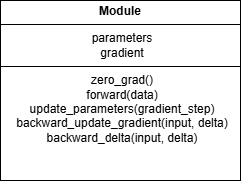
\includegraphics[width=0.4\linewidth]{Images/module.png}
    \caption{Diagramme de la classe Module}
    \label{fig:module}
\end{figure}

La majorité des fonctions de cette classe ne sont pour l'instant pas implémentées, à l'exception des méthodes $zero\_grad$ et $update\_parameters$. Ainsi, dans la première, on commence par vérifier si la variable gradient n'est pas nulle, afin de s'assurer de pouvoir la manipuler. Si elle existe bien, on met à jour cette variable en mettant un zéro pour chaque paramètre contenu dans notre variable $parameters$. 
Dans $update_parameters$, on commence par vérifier cette fois-ci si les deux variables de notre classe sont bien définies, puis on met à jour la variable $parameters$ en soustrayant le vecteur de la variable $gradient$ à celui de nos paramètres, en veillant bien à multiplier celui-ci par le pas de gradient en paramètres.
Le reste des méthodes seront implémentées dans les classes filles qui héritent de cette classe abstraite.

\subsection{Classe Loss}
Cette seconde classe abstraite nous permet donc de disposer des méthodes pour implémenter les différentes fonction de perte que nous souhaiterions utiliser dans notre réseau de neurones. Elle ne dispose que de deux méthodes : $forward$, qui prend en paramètre deux entrées et calcule le coût, et la méthode $backward$, qui va nous permettre de calculer le coup du gradient par rapport à une entrée. Il n'y a donc pas besoin de les implémenter pour l'instant : il faudra le faire spécifiquement en fonction des fonctions de coûts que nous souhaitons mettre en place.

\section{Mon premier est ... linéaire !}
\subsection{Implémentation de la perte MSE}
On commence donc par implémenter la fonction de perte Mean Squared Error (MSE), qui est la fonction la plus couramment utilisée pour les régressions linéaires.\[
\text{MSE}(y, \hat{y}) = (y_i - \hat{y}_i)^2
\]
où \(y\) est le vecteur des valeurs réelles, \(\hat{y}\) est le vecteur des prédictions, et \(n\) est le nombre d'échantillons. Pour ceci, on commence par déclarer la méthode \textbf{forward}, qui va nous permettre de calculer la perte entre les deux vecteurs d'entrée. On commence par vérifier que les deux vecteurs sont bien de la même taille, puis on calcule la somme des carrés des différences entre les deux vecteurs, on pourra ainsi calculer la moyenne dans notre descente de gradient. On récupère ainsi notre perte. On implémente ensuite la méthode backward, qui correspond au calcul de gradient de notre perte, s'exprimant ainsi :
\[
\frac{\partial \text{MSE}}{\partial \hat{y}} = -{2} (y - \hat{y})
\]
Cela va nous permettre d'obtenir les valeurs des gradients de notre perte et donc de pouvoir effectuer notre backpropagation.

La classe \texttt{MSELoss} hérite de la classe \texttt{Loss} et implémente les méthodes \texttt{forward} et \texttt{backward} pour calculer respectivement la perte et le gradient.

\subsection{Implémentation du module linéaire}

Le module linéaire, est une brique fondamentale de notre implémentation de réseau de neurones. Celle-ci hérite de la classe \textbf{Module}, et possède comme paramètre une matrice de poids de de dimension entrée/sortie. On ajoute une dimension de plus en entrée qui correspond à un vecteur de biais, facilitant l'implémentation de celui-ci. Pour la variable $gradient$, on crée une matrice remplie de zéro de la même taille.

Pour la méthode \textbf{forward}, on commence donc par ajouter un vecteur unitaire de biais dans nos données X, grâce à la fonction \textbf{hstack}. On effectue ensuite le produit matricielle grâce à l'opérateur $@$, qui est équivalent à la fonction \textbf{np.dot}.\\
On passe ensuite à la méthode \textbf{backward-update-gradient}, dans laquelle on commence par vérifier les bonnes dimensions de nos paramètres, mais aussi par ajouter un vecteur unitaire pour le biais. On ajoute ensuite notre gradient, obtenu par produit matriciel, dans la variable $self.gradient$.

\subsection{Expérimentation : Régression linéaire}

Avec ces deux éléments, nous pouvons maintenant implémenter une régression linéaire simple. Nous entraînerons un modèle pour prédire une sortie à partir d'une entrée donnée, en minimisant la perte MSE. Les premières expérimentations s'effectuent ainsi sur une simple fonction linéaire de la forme : $y=3x+4$. Comme pour toutes les expérimentations dans ce projet, nous prenons soin de séparer les données d'entraînement et de test, afin de pouvoir évaluer la performance de notre modèle sur des données non vues, et donc d'éviter un phénomène de surapprentissage. Nous utilisons la fonction \textbf{train\_test\_split} de la bibliothèque \textbf{sklearn} pour cela.

On dresse ainsi un graphique montrant la valeur de la perte en fonction du nombre d'itérations, ainsi qu'un second graphique montrant la valeur de la sortie prédite par rapport à la sortie réelle. On peut voir que la perte fini bien par converger, et que les valeurs prédites sont très proches des valeurs réelles. \ref{fig:res_reg_lin}.

\begin{figure}[H]
    \centering
    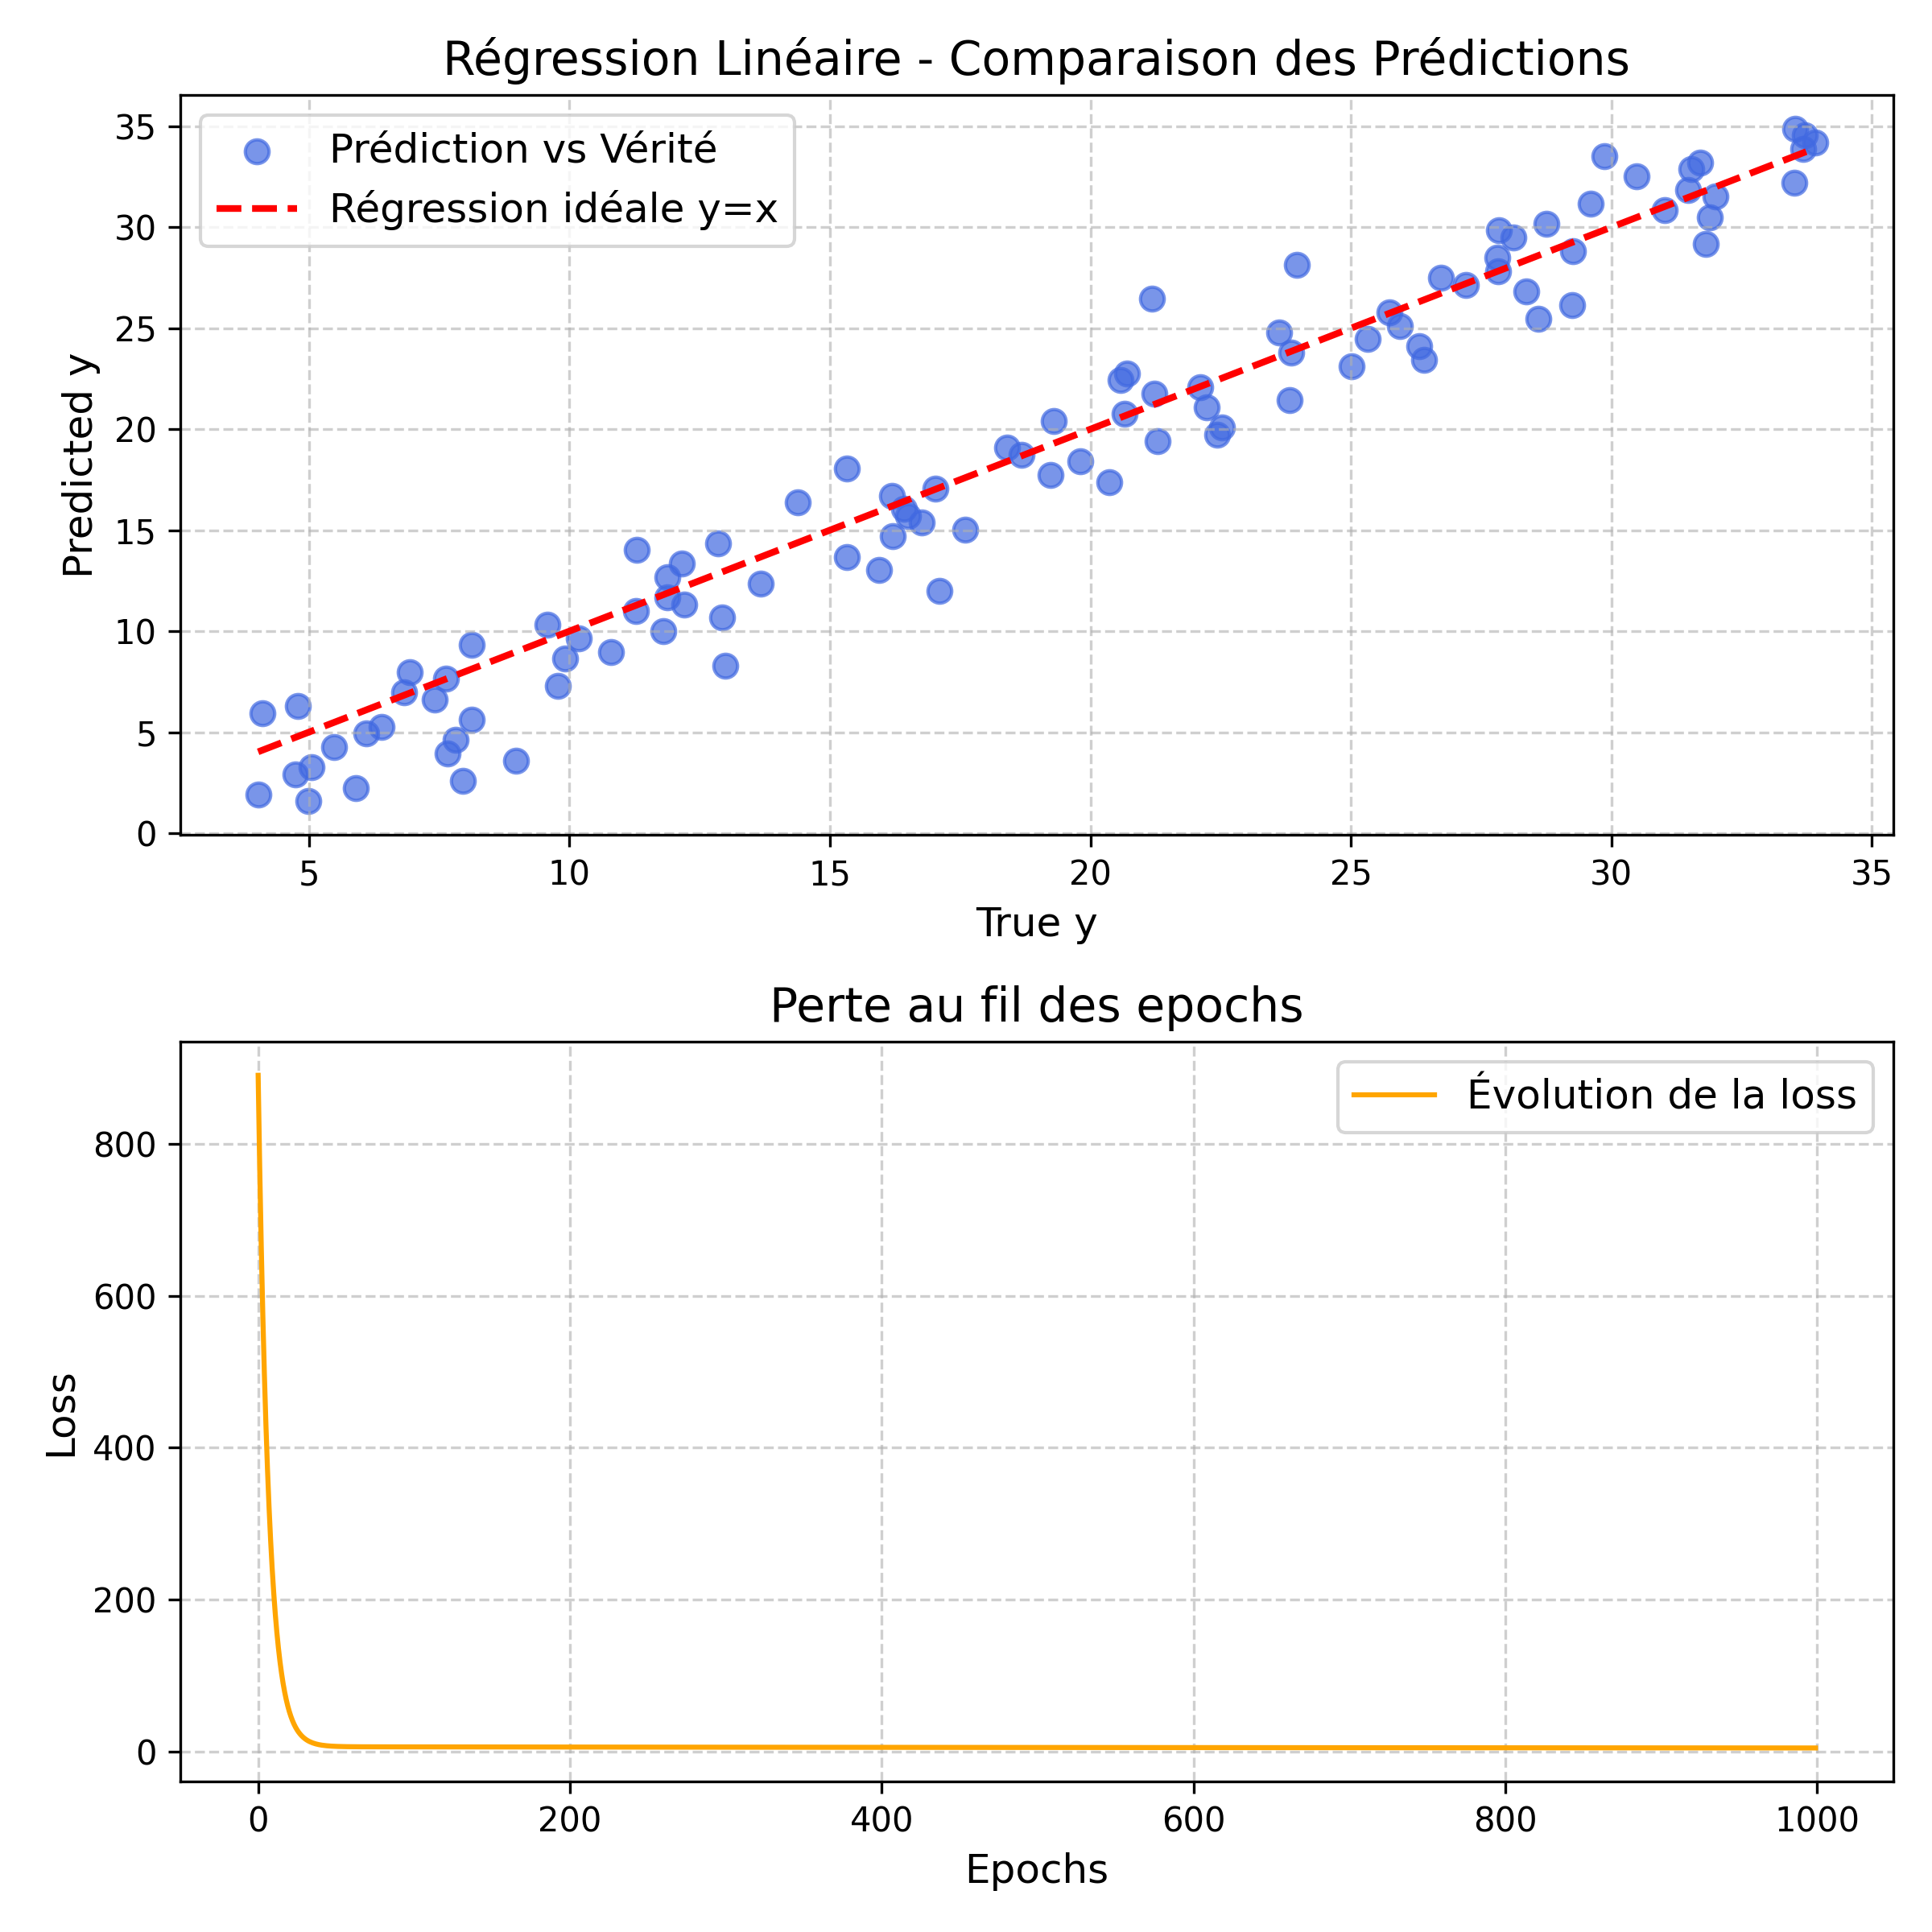
\includegraphics[width=0.8\linewidth]{Images/regression_lineaire.png}
    \caption{Loss et prédictions de la régression linéaire}
	\label{fig:res_reg_lin}
\end{figure}

On teste ensuite sur différents problèmes de classification, en utilisant la fonction \textbf{gen\_arti} que nous avons déjà utilisé dans les différents TMEs de l'UE. On a donc trois jeux de données : le premier étant un mélange de deux gaussiennes, le deuxième un mélange de 4 gaussiennes (XOR), et enfin un échiquier. Les résultats de la classification sont visiles dans la figure \ref{fig:res_classif_reg_lin}.

\begin{figure}[H]
    \centering
    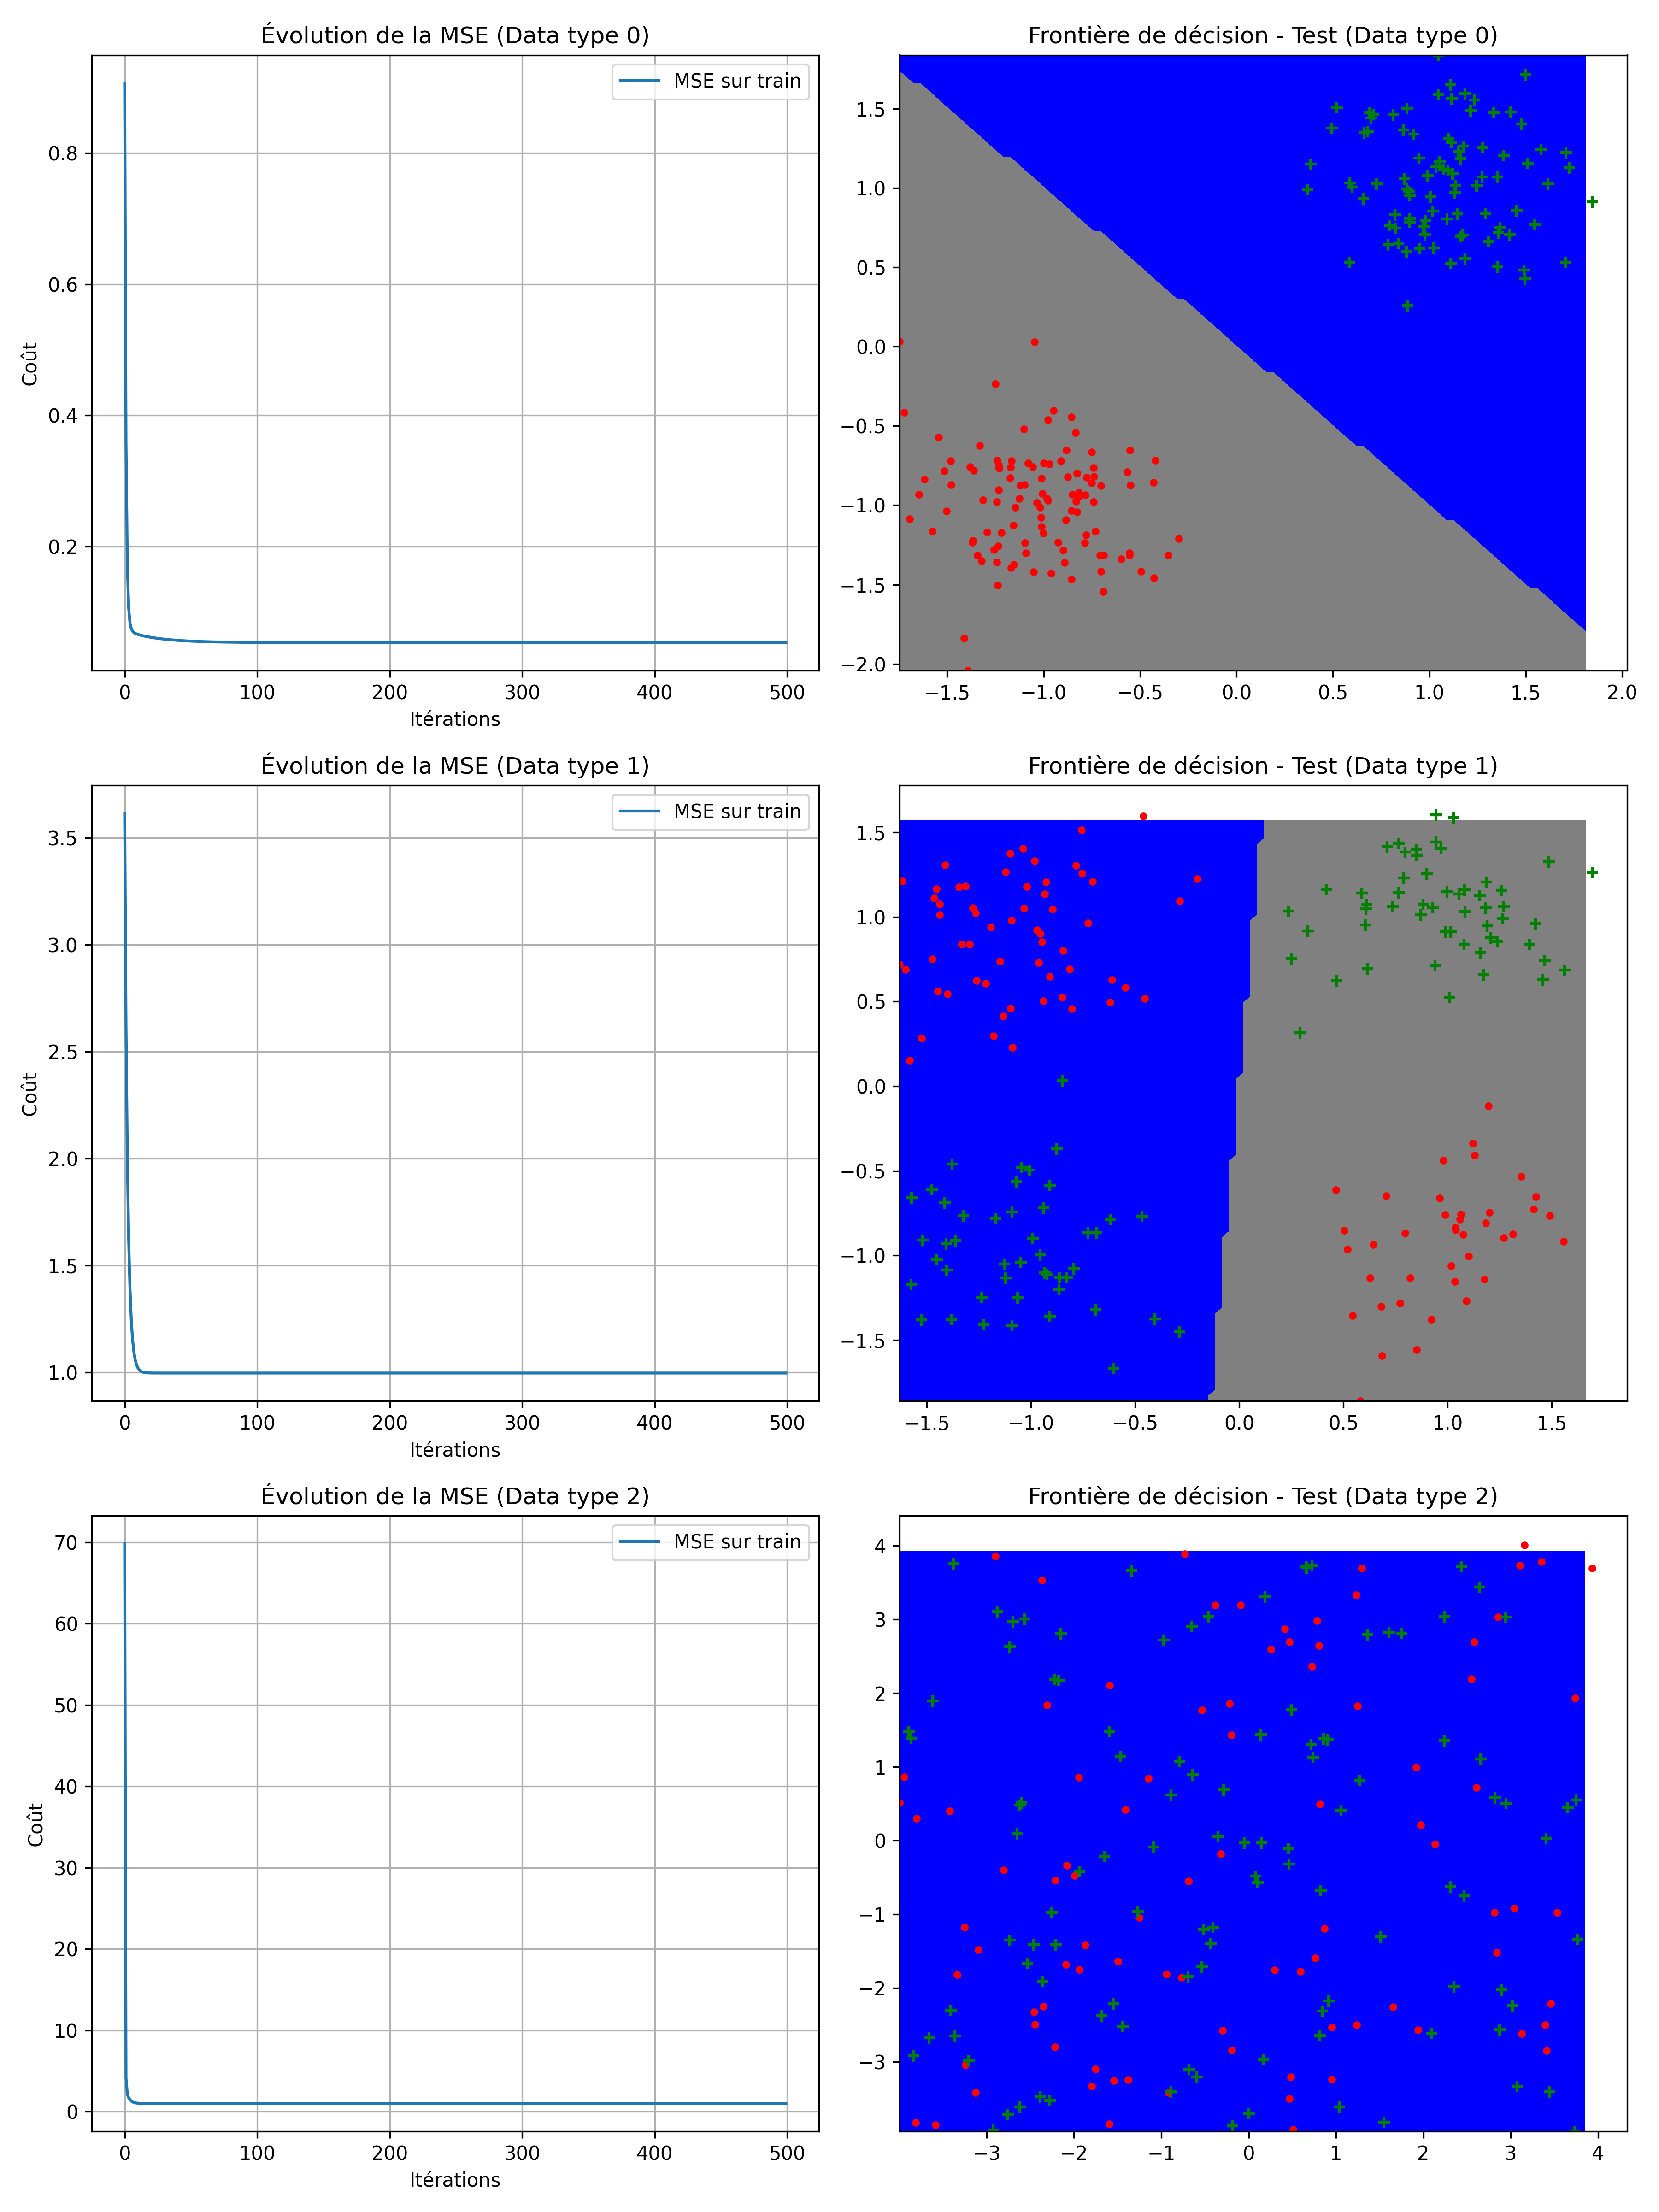
\includegraphics[width=0.8\linewidth]{Images/classif_reg_lineaire.png}
    \caption{Loss et prédictions de la régression linéaire}
	\label{fig:res_classif_reg_lin}
\end{figure}

On peut donc voir que la régression linéaire fonctionne bien sur la séparation des deux gaussiennes, ce qui est logique puisque la séparation est linéaire. Pour les 4 gaussiennes, la loss converge vers des valeurs beaucoup plus haute, une régression linéaire simple ne pouvant pas suffire à résoudre un tel problème, ce qui est encore plus visible sur notre problème d'échiquier.

\section{Mon second est ... non linéaire !}
\subsection{Implémentations}
Nous commençons par implémenter la fonction d’activation \textbf{TanH}, qui hérite de la classe \texttt{Module}. Il suffit pour cela d’implémenter la méthode \texttt{forward}, qui applique simplement la fonction $\tanh$ de la bibliothèque \texttt{numpy}. La méthode \texttt{backward\_delta}, quant à elle, permet de calculer le gradient de l’activation en utilisant la dérivée de la tangente hyperbolique :

\[
\delta = \delta \times \left(1 - \tanh^2(X)\right)
\]

Pour la fonction sigmoïde, l’implémentation suit le même principe, seulement il n’existe pas de fonction sigmoïde prédéfinie dans \texttt{numpy}. Il faut donc la définir explicitement :

\[
\sigma(X) = \frac{1}{1 + e^{-X}}
\]

La dérivée est ensuite utilisée dans la méthode \texttt{backward\_delta} :

\[
\delta = \delta \times \sigma(X) \times \left(1 - \sigma(X)\right)
\]



Enfin, afin de tester notre premier réseau de neurones, nous avons mis en place la classe \textbf{SimpleNN}, qui va nous permettre de créer un réseau constitué d'une couche linéaire, puis d'une fonction d'activation \textbf{tanh}, puis d'une seconde couche linéaire et enfin d'une fonction \textbf{sigmoide}. On implémente la méthode \textbf{forward}, qui va nous permettre de faire passer nos données dans le réseau, en appelant les différentes méthodes \textbf{forward} de chaque module, en prenant en paramètre le retour de la fonction forward de la couche précédente. Pour la méthode \textbf{backward}, on commence par calculer le gradient de la loss, puis on va calculer tous les deltas dont nous avons besoin par rétropropagation, en appelant la méthode \textbf{backward\_delta} de chaque module, en prenant en paramètre le retour de la fonction backward de la couche suivante. Enfin, on appelle la méthode \textbf{backward\_gradient\_update} sur chacune des couches linéaires. Pour les deux autres méthodes que sont \textbf{zero\_grad} et \textbf{update\_parameters}, on appelle simplement la méthode de la classe mère pour chacune des couches linéaires.
\subsection{Expérimentation : Réseau de neurones simple}

On teste donc sur les mêmes jeux de données que précédemment, mais cette fois-ci avec un réseau de neurones simple, constitué d'une couche linéaire, d'une fonction d'activation \textbf{tanh}, d'une seconde couche linéaire et enfin d'une fonction \textbf{sigmoide}. Les résultats sont visibles dans la figure \ref{fig:simplenn}.

\begin{figure}[H]
    \centering
    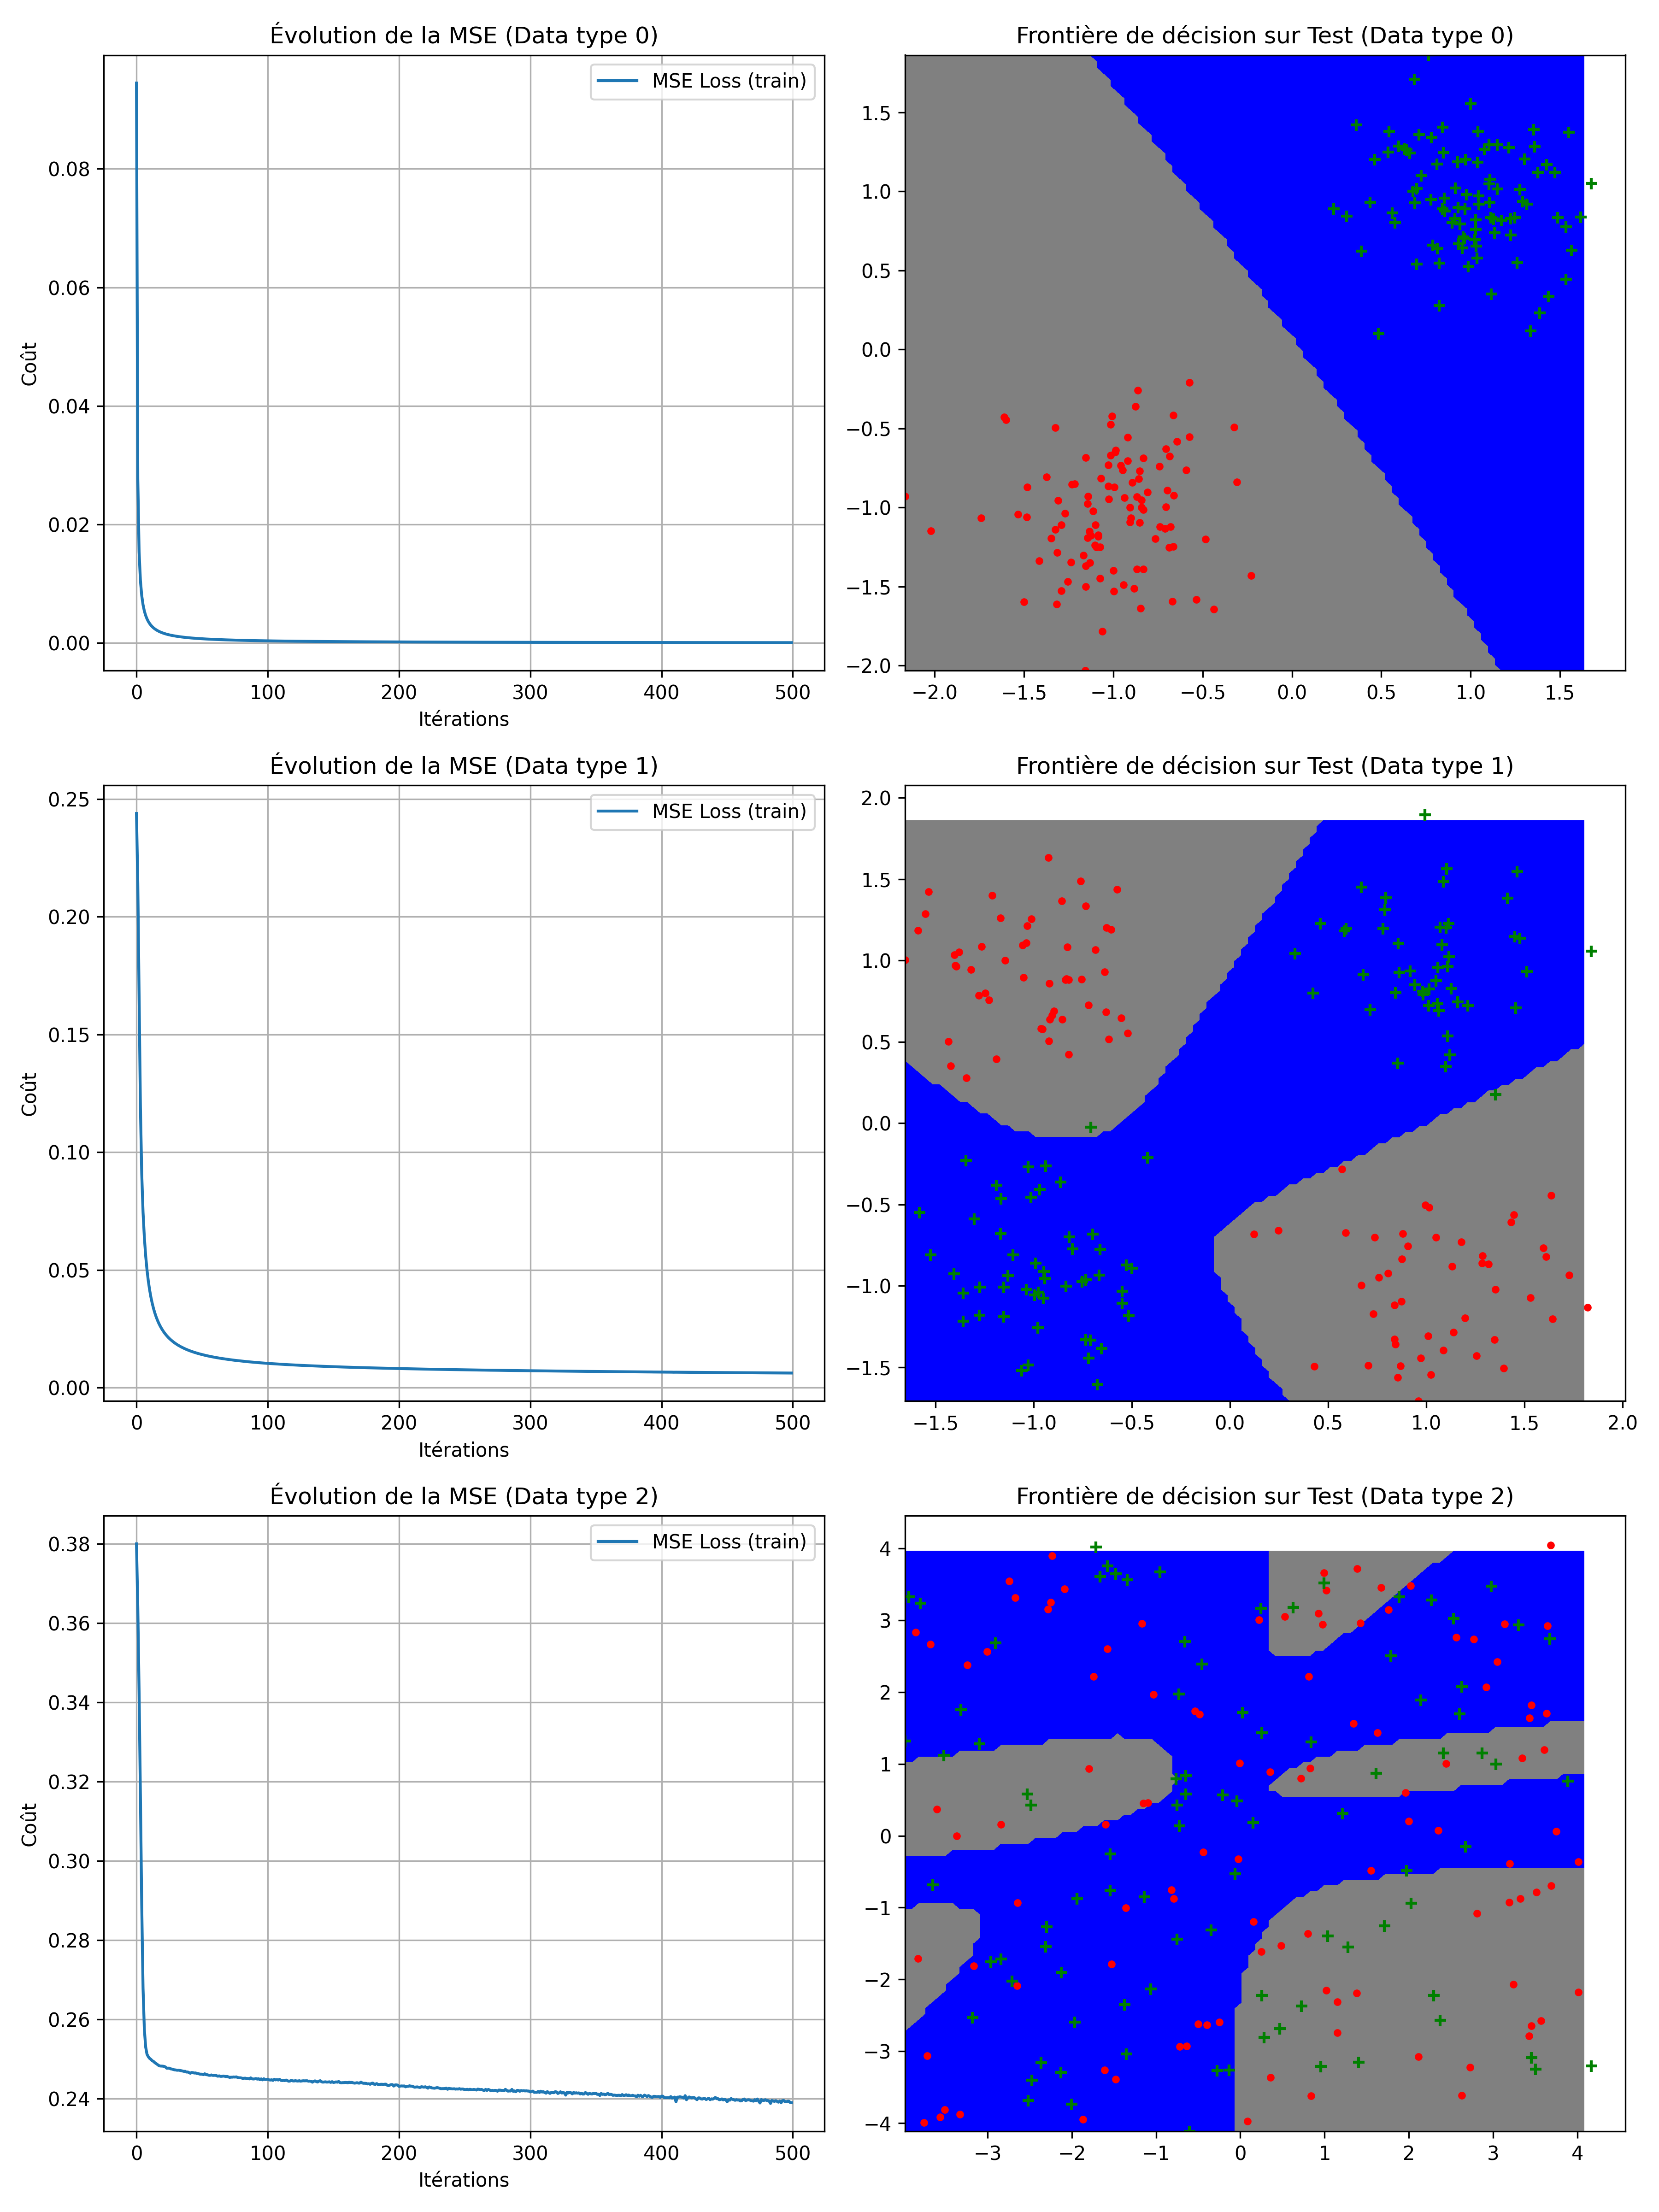
\includegraphics[width=0.8\linewidth]{Images/sigmoide_tanh_combined.png}
    \caption{Loss et frontières avec une couche cachée}
	\label{fig:simplenn}
\end{figure}

On peut voir que la loss converge bien plus rapidement que pour la régression linéaire, et que les résultats sont bien meilleurs. On peut voir que le réseau arrive à bien séparer les deux gaussiennes, mais aussi le XOR. En revanche, il n'arrive pas à séparer l'échiquier, ce problème nécessitant de mettre en place un réseau avec plus de couches.

\section{Mon troisième est un encapsulage}
\subsection{Classe Sequentiel}
Pour la classe \textbf{Sequentiel}, on suit le même principe que pour la classe \textbf{SimpleNN}, mais cette fois en généralisant afin de pouvoir construire un réseau de neurones plus grand. Cette classe ne possède ainsi qu'un seul paramètre, une liste de modules. Pour la méthode \textbf{forward}, on parcours donc notre liste en faisant appel à cette même méthode pour chacun des modules du réseau. Pour la \textbf{backward}, on parcours la liste dans le sens inverse, et on update les gradients de chacune des couches linéaires, en calculant également les gradients de delta. Pour les deux dernières méthodes, on appelle simplement la méthode de la classe mère pour chacune des couches linéaires.

Pour expérimenter notre réseau, on teste à la fois sur les mêmes données que précédemment, mais aussi sur d'autres répartition de données, afin de mettre en avant l'efficacité de notre implémentation. De plus, on compare l'évolution de la loss en entraînement ainsi que la frontière de décision avec la bibliothèque \textbf{PyTorch}, afin de voir si notre implémentation est correcte. Les résultats sont visibles dans les figures suivantes. On teste ici avec 500 épochs, avec une batch size de 32.
\begin{figure}[H]
    \centering
    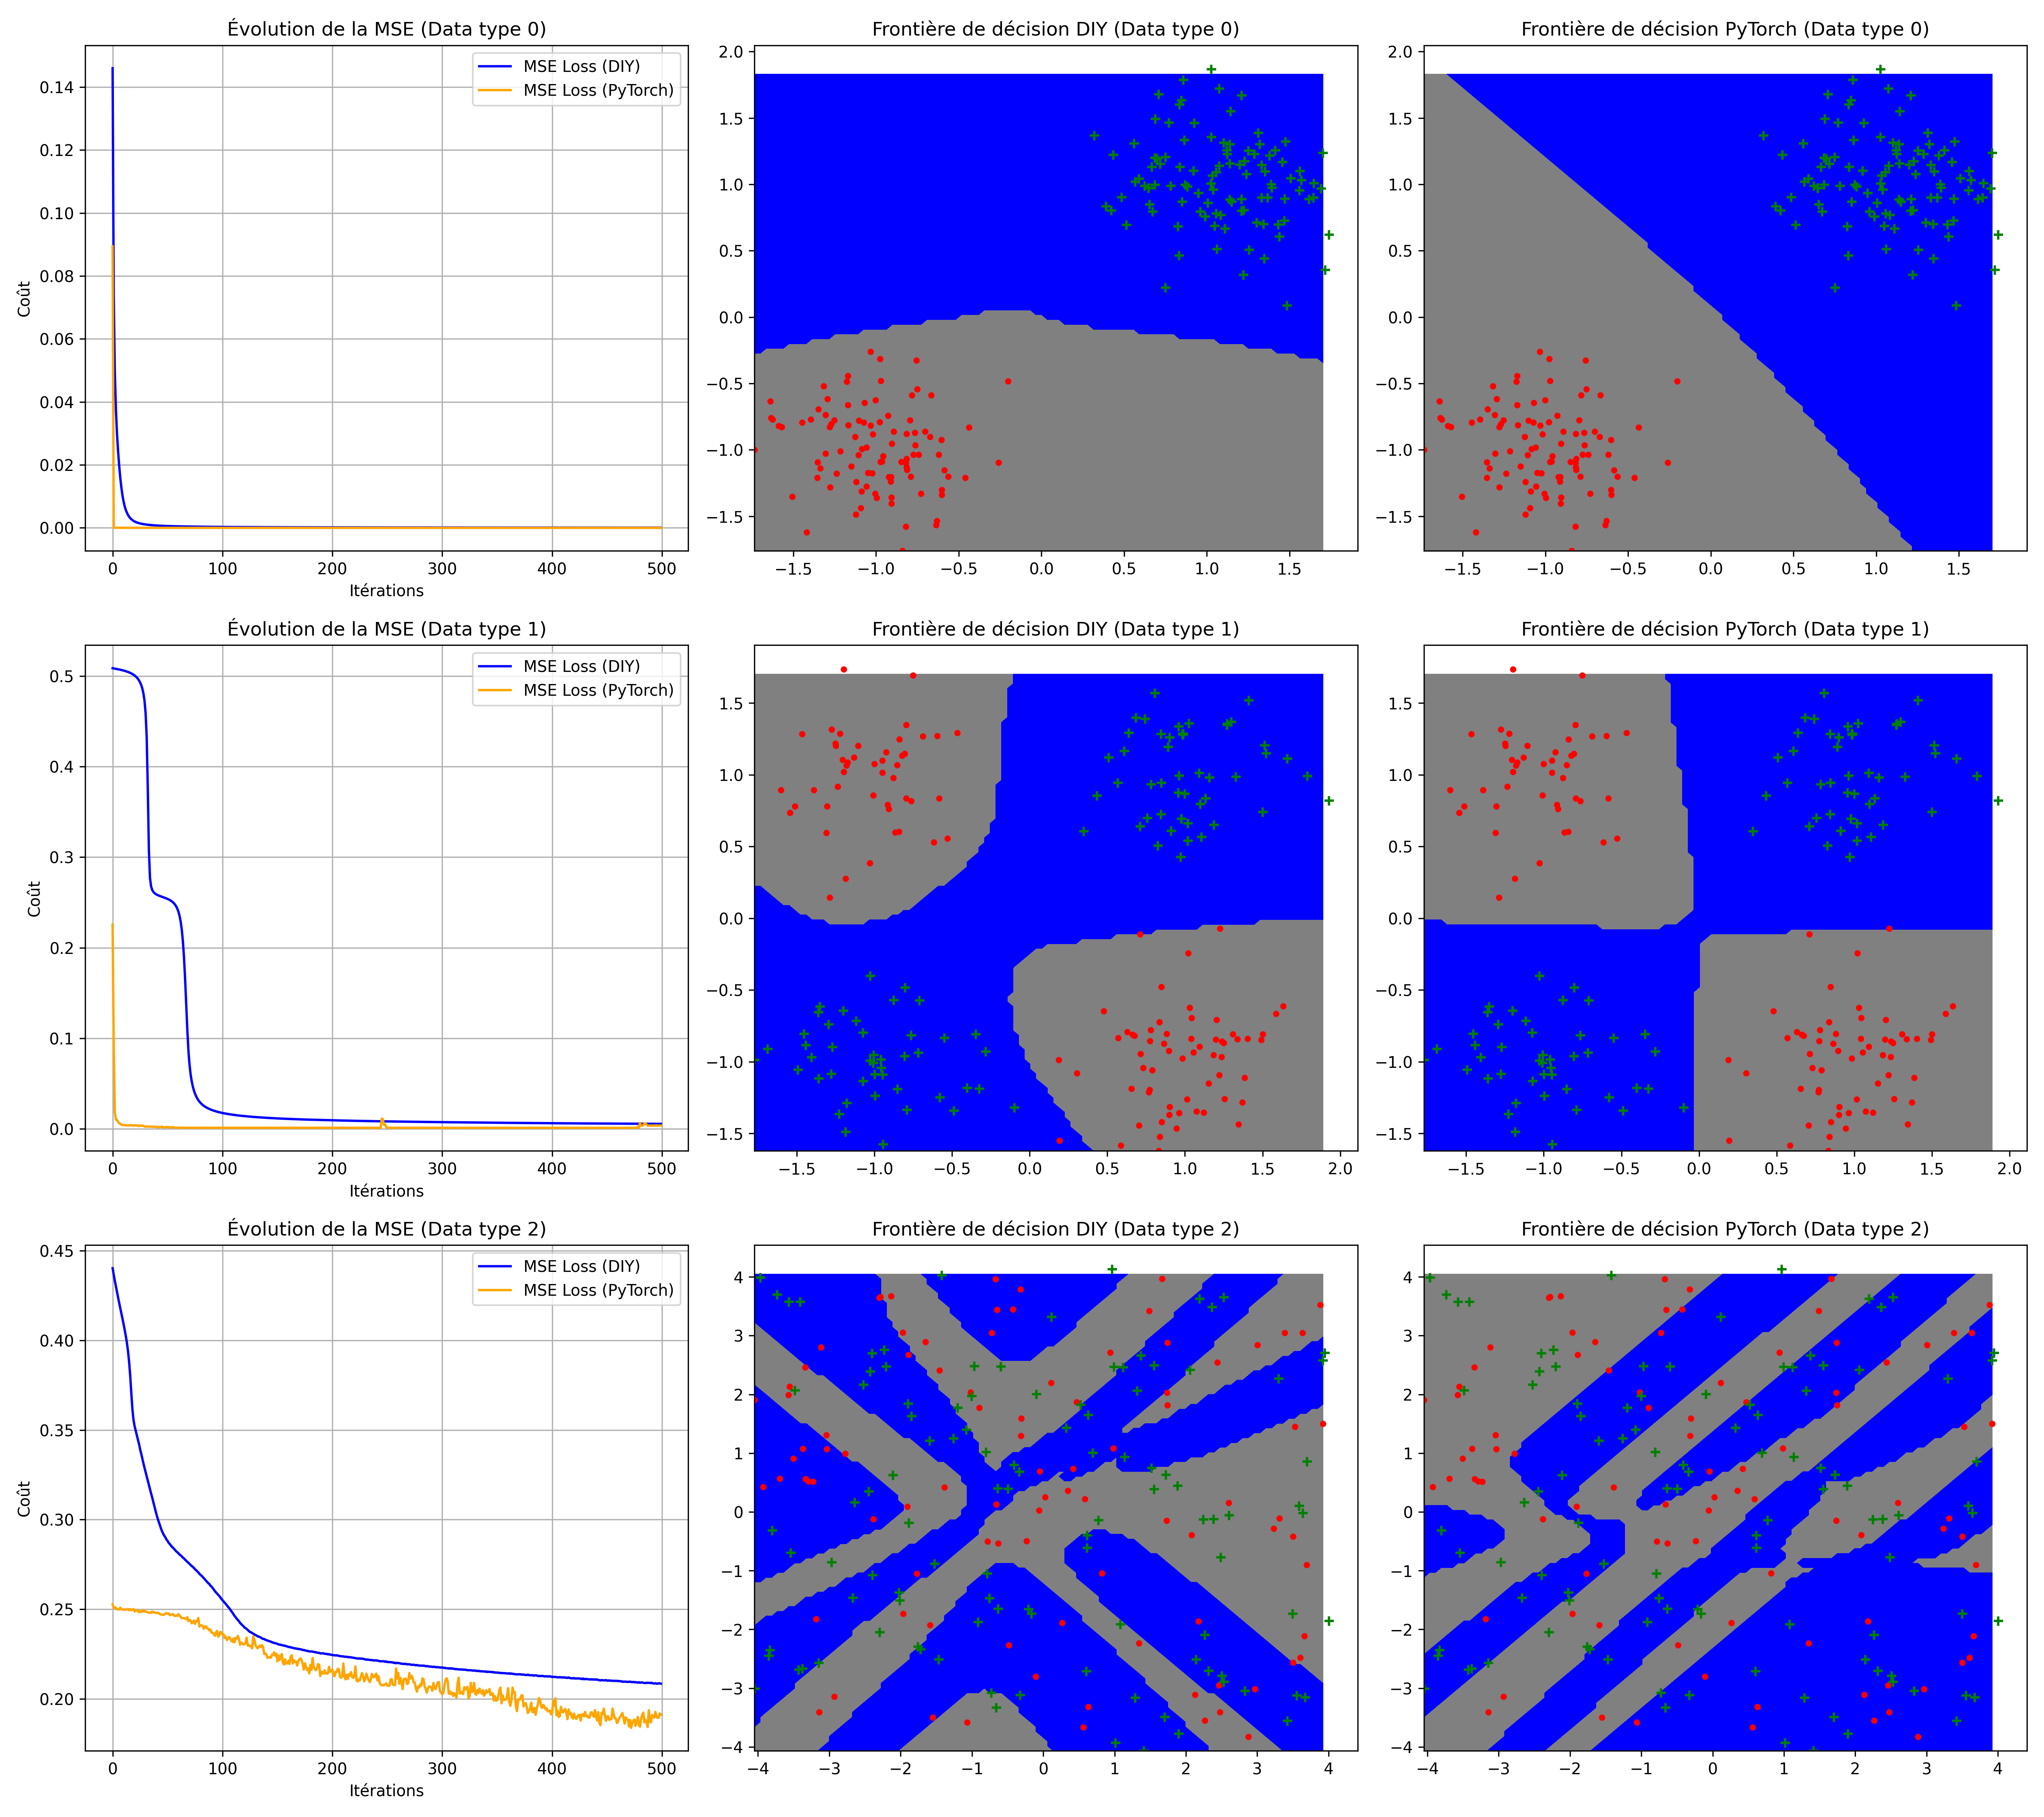
\includegraphics[width=0.8\linewidth]{Images/sequentiel_1.png}
    \caption{Loss et frontières avec la classe Sequentiel (premières données)}
	\label{fig:sequentiel1}
\end{figure}
On teste ici avec un réseau constitué de la manière suivante : Une couche linéaire (2,5), puis une autre de (5,10), (10,20), puis (20,1), en séparant les couches internes par des fonction de tangente hyperbolique, et en ajoutant une fonction sigmoide à la fin.
On remarque que la loss converge bien plus rapidement que pour le réseau de neurones simple, et que les résultats sont bien meilleurs. On peut voir que le réseau arrive à bien séparer les deux gaussiennes, mais aussi le XOR. En revanche, il n'arrive pas à séparer l'échiquier, ce problème nécessitant probablement de mettre en place un réseau avec plus de couches.
La différence d'évolution entre la loss du réseau DIY et la loss de PyTorch est peut-être due à la non utilisation d'optimiseur pour l'instant, point que nous verrons dans la partie suivante.
\begin{figure}[H]
    \centering
    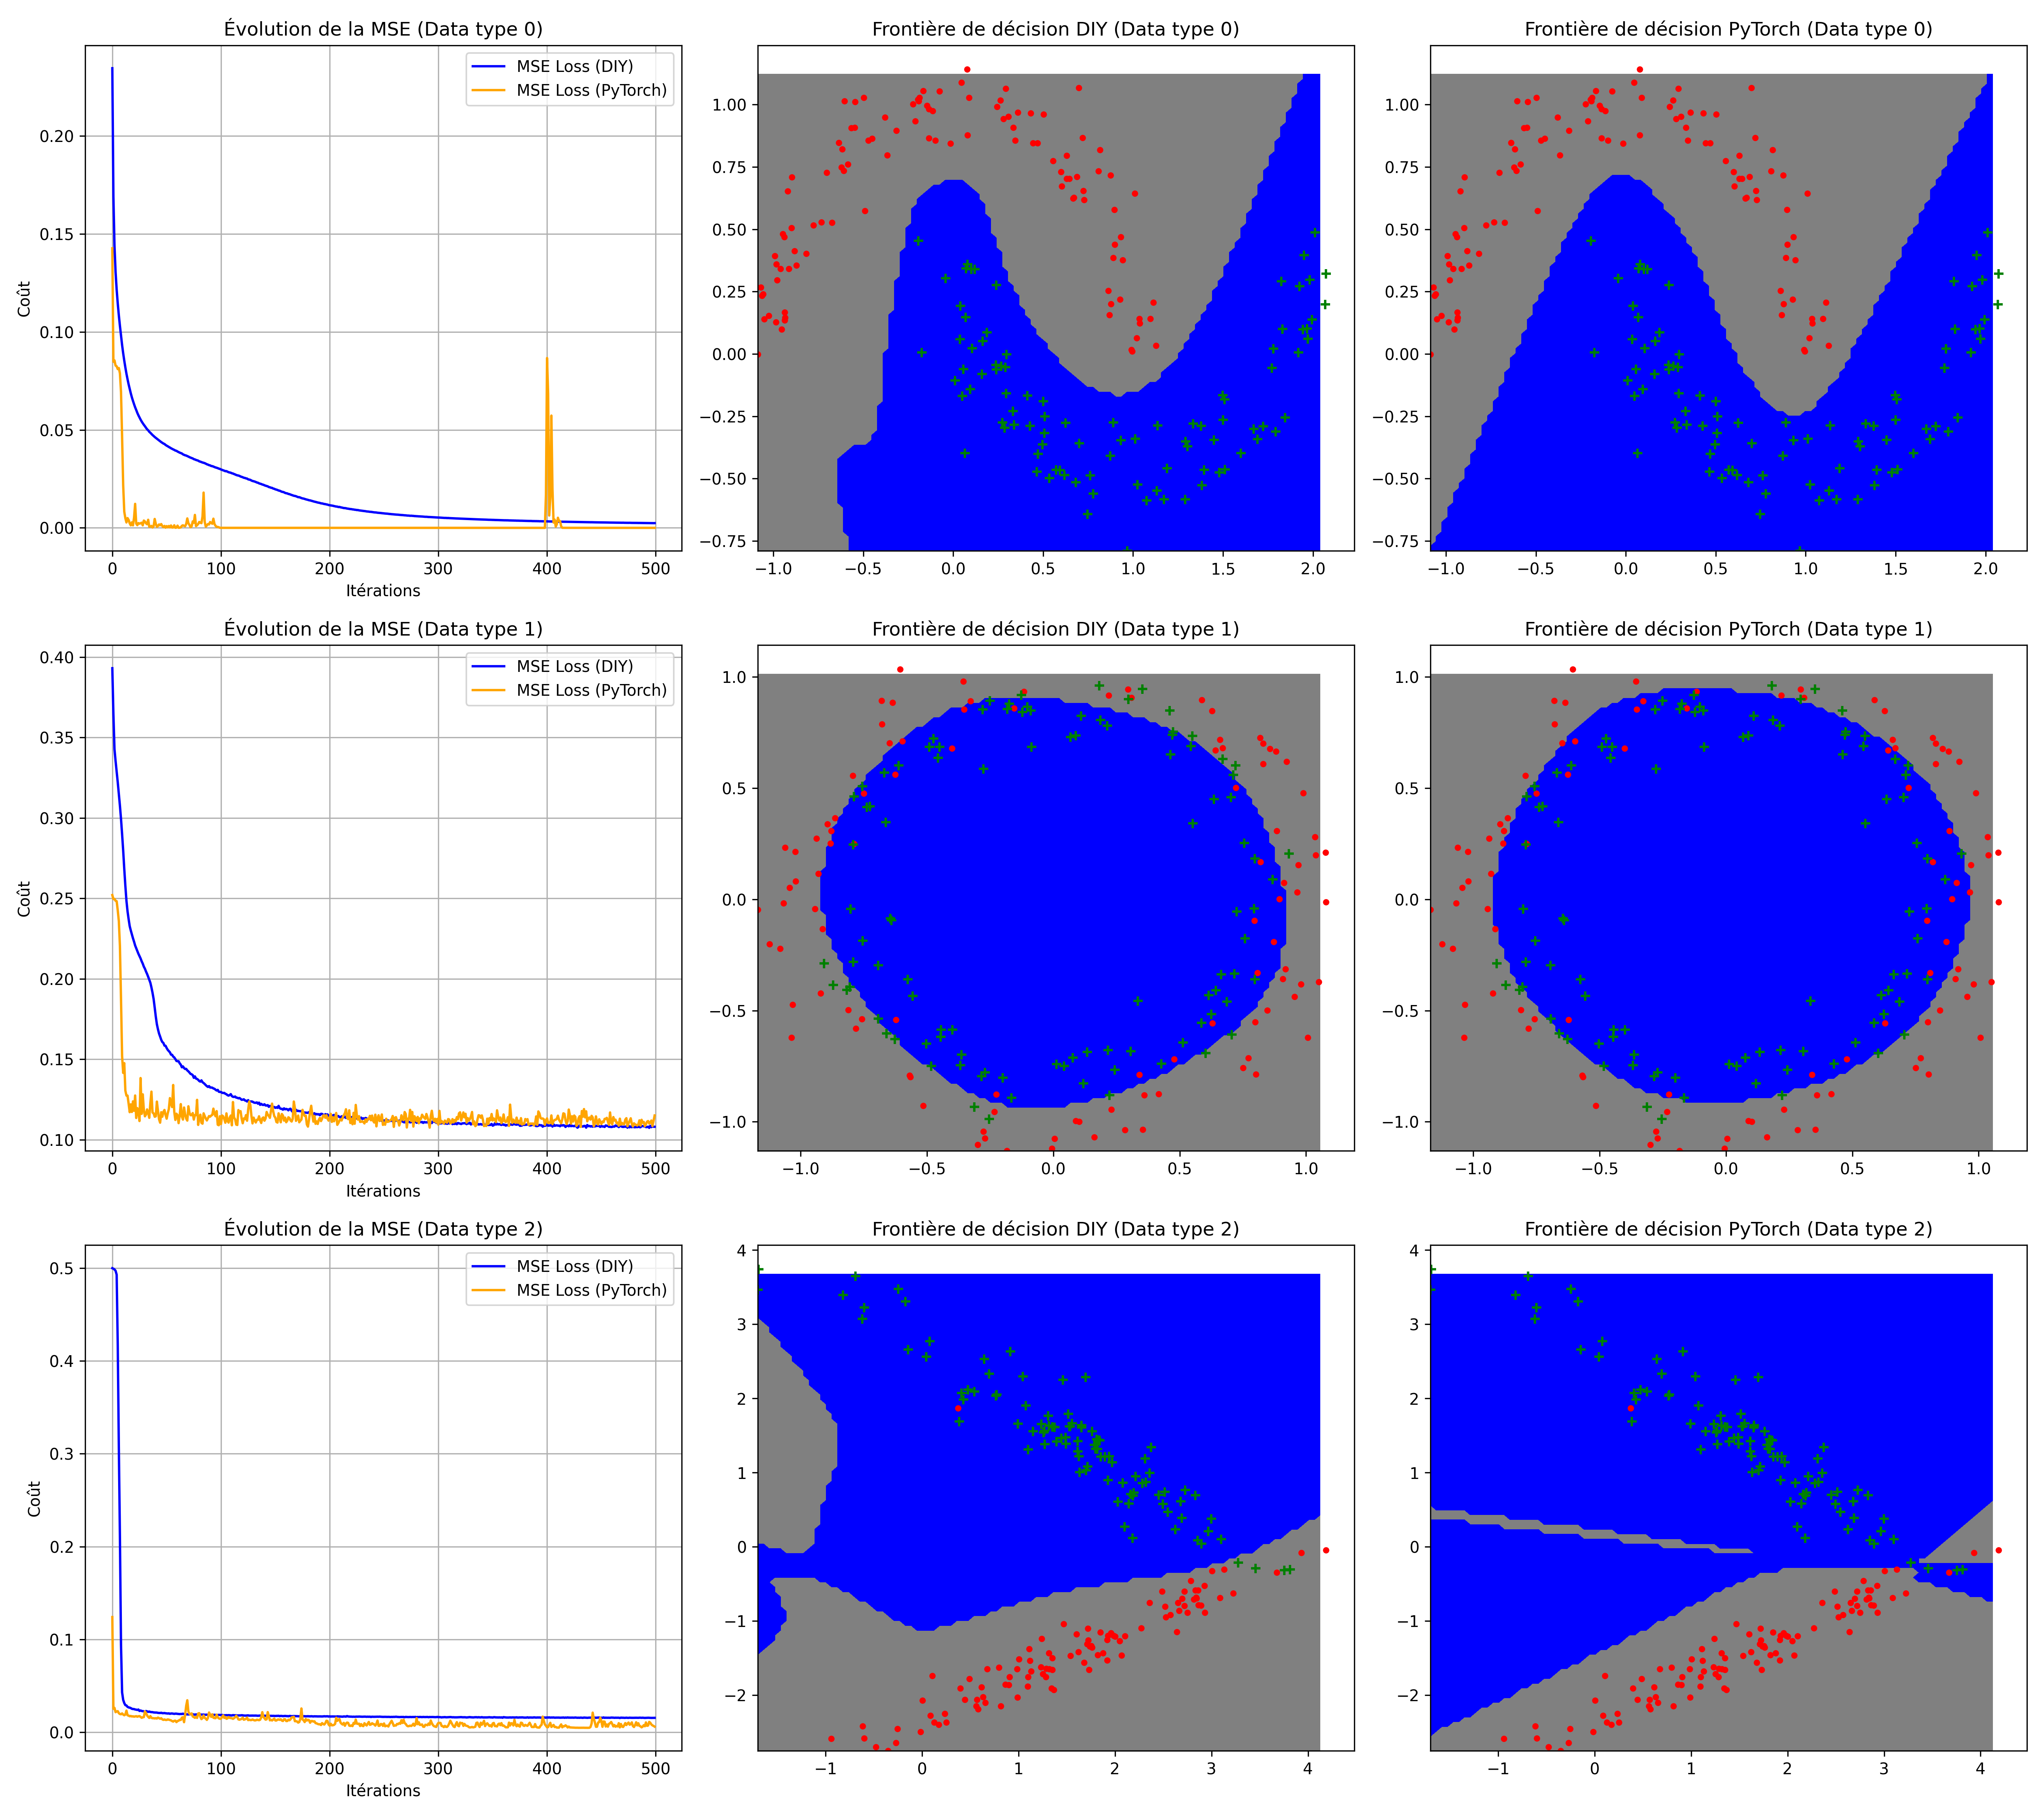
\includegraphics[width=0.8\linewidth]{Images/sequentiel_2.png}
    \caption{Loss et frontières avec la classe Sequentiel (secondes données)}
	\label{fig:sequentiel2}
\end{figure}
Avec le même réseau, on arrive ici à résoudre des problèmes de classification plus complexes que nos deux premiers, témoignant de l'efficacité des réseaux de neurones.
\subsection{Optim et SGD}
Afin de nous rapprocher le plus possible de la bibliothèque \textbf{PyTorch}, on met en place la classe \textbf{Optim}, conformément aux informations de l'énoncé. On impémente également la fonction SGD, qui correspond à la fonction de train que nous utilisions précedemment en utilisant cette fois-ci notre optimiseur.
On expérimente ainsi sur les mêmes données que précedemment, dont les résultats sont visibles dans la figure \ref{fig:optim1} et \ref{fig:optim2}.
\begin{figure}[H]
    \centering
    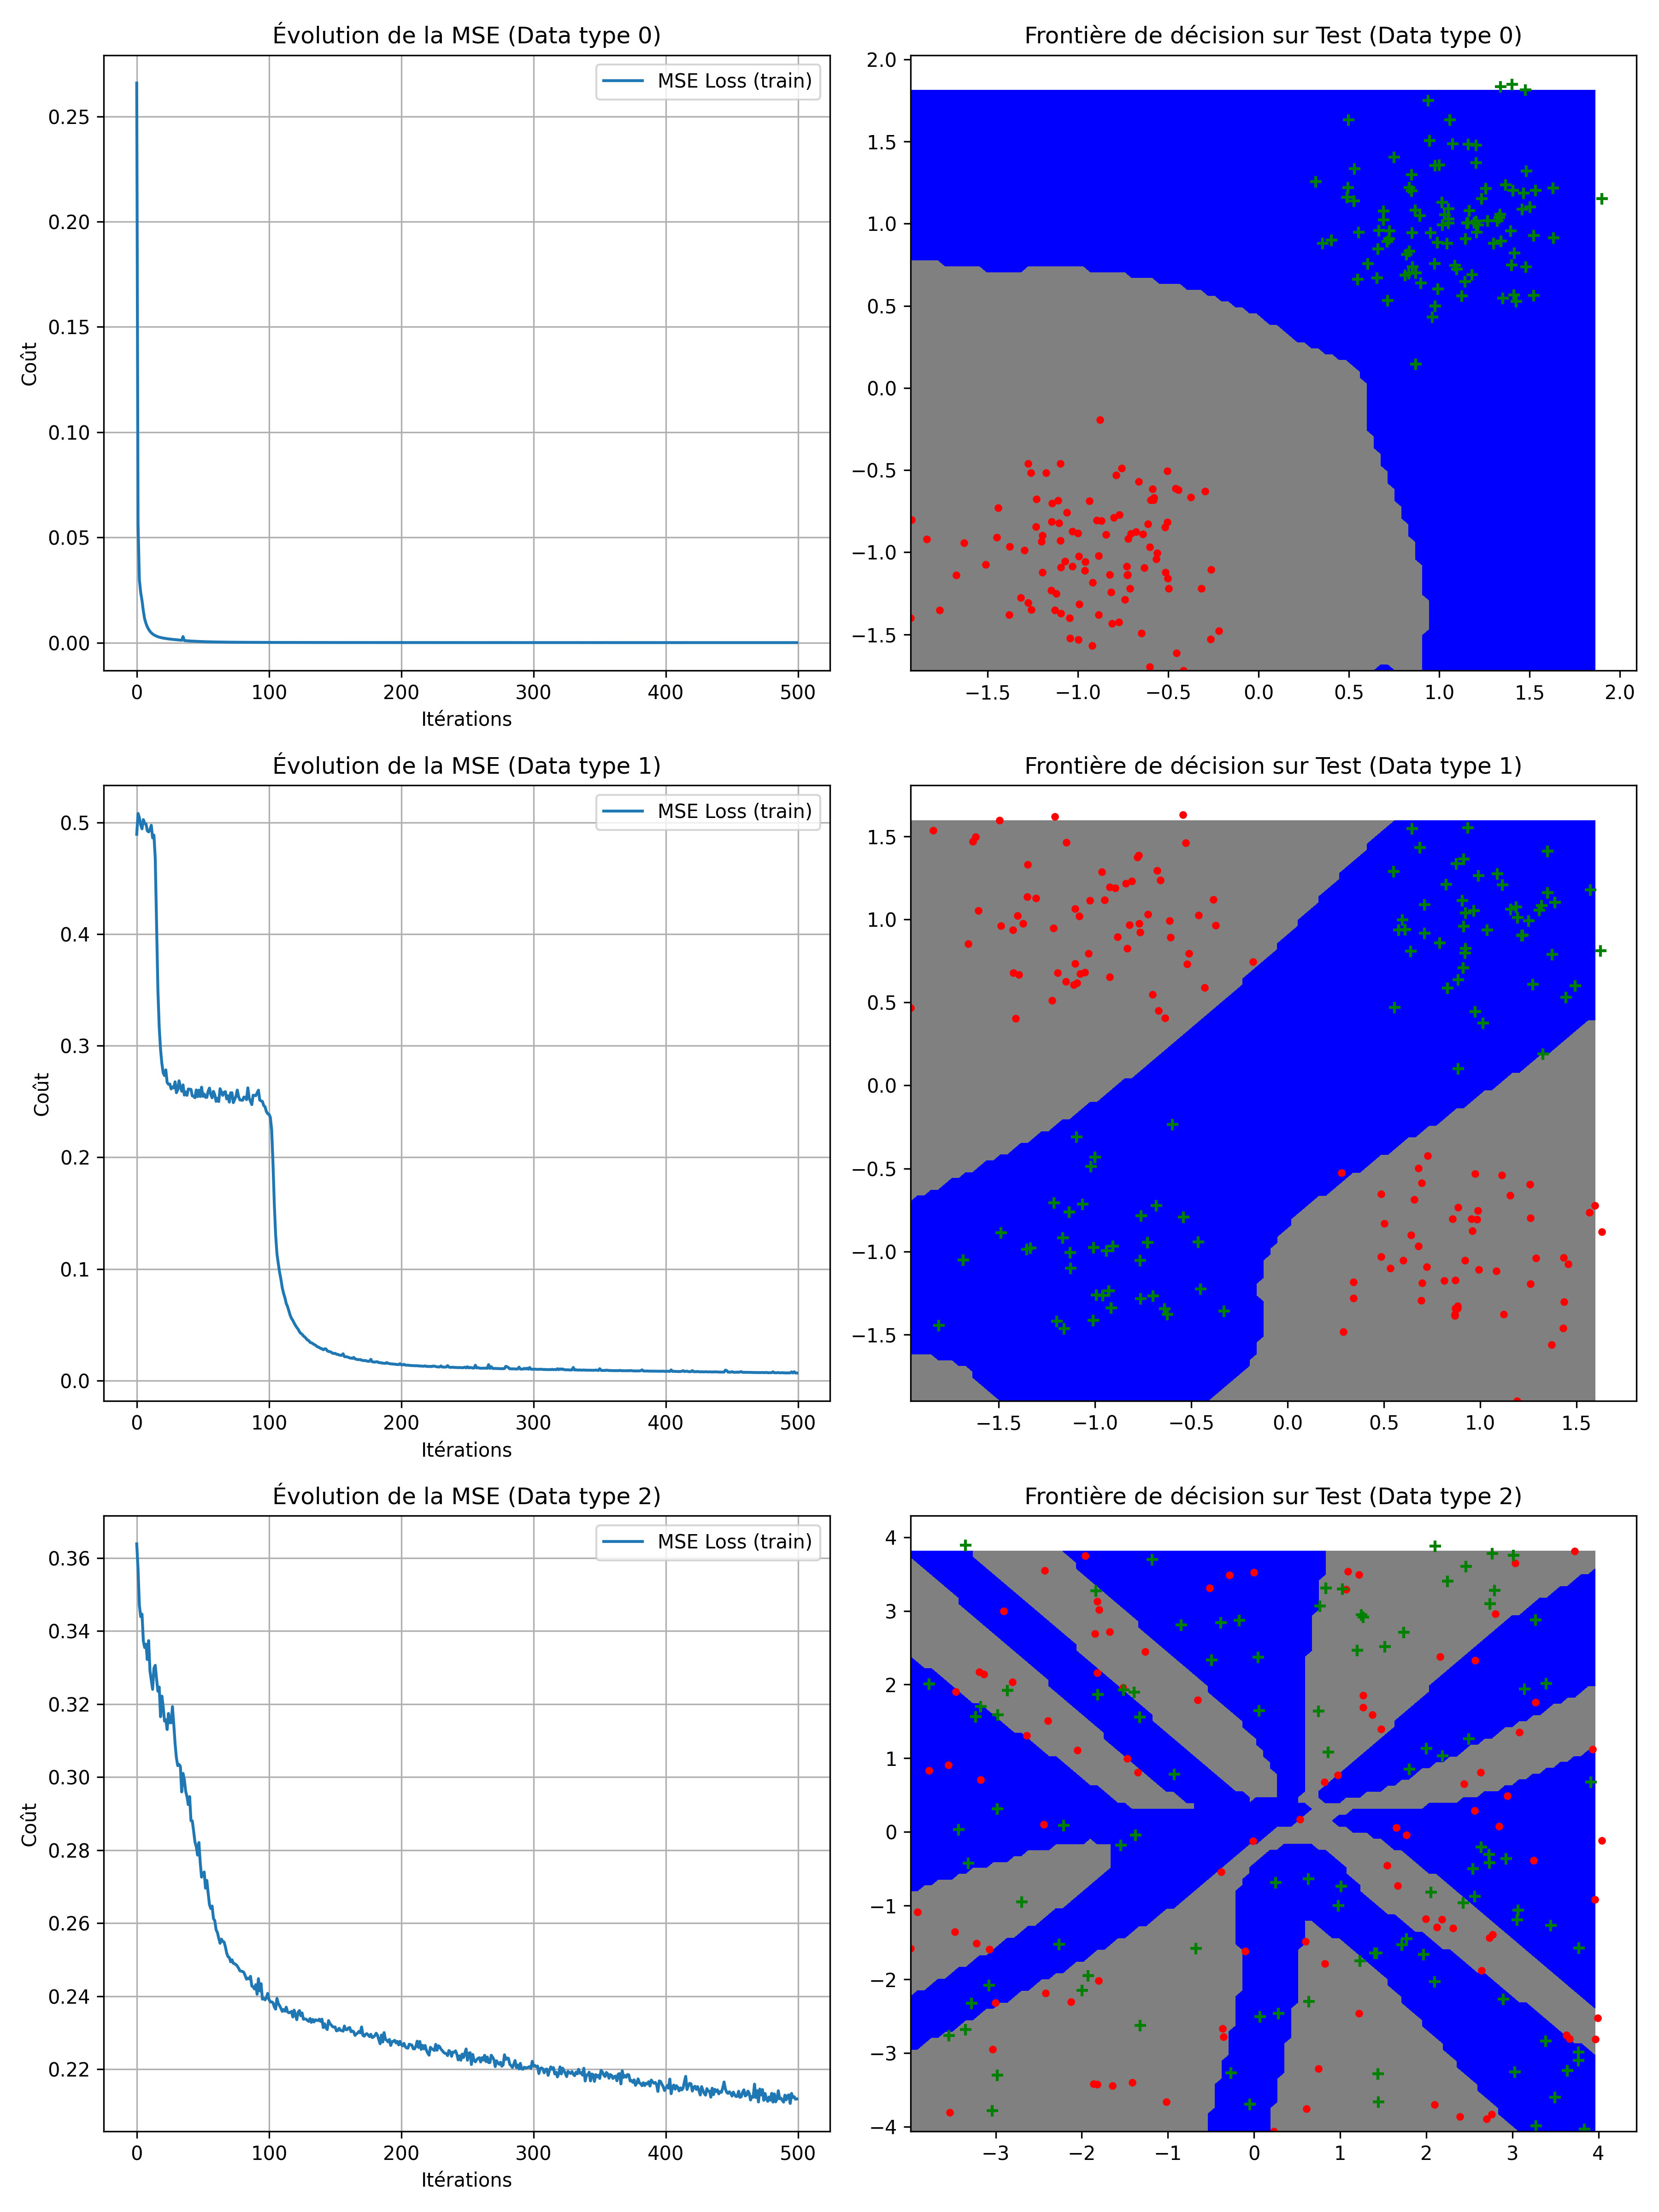
\includegraphics[width=0.8\linewidth]{Images/optim1.png}
    \caption{Loss et frontières avec optimisation  (premières données)}
	\label{fig:optim1}
\end{figure}

\begin{figure}[H]
    \centering
    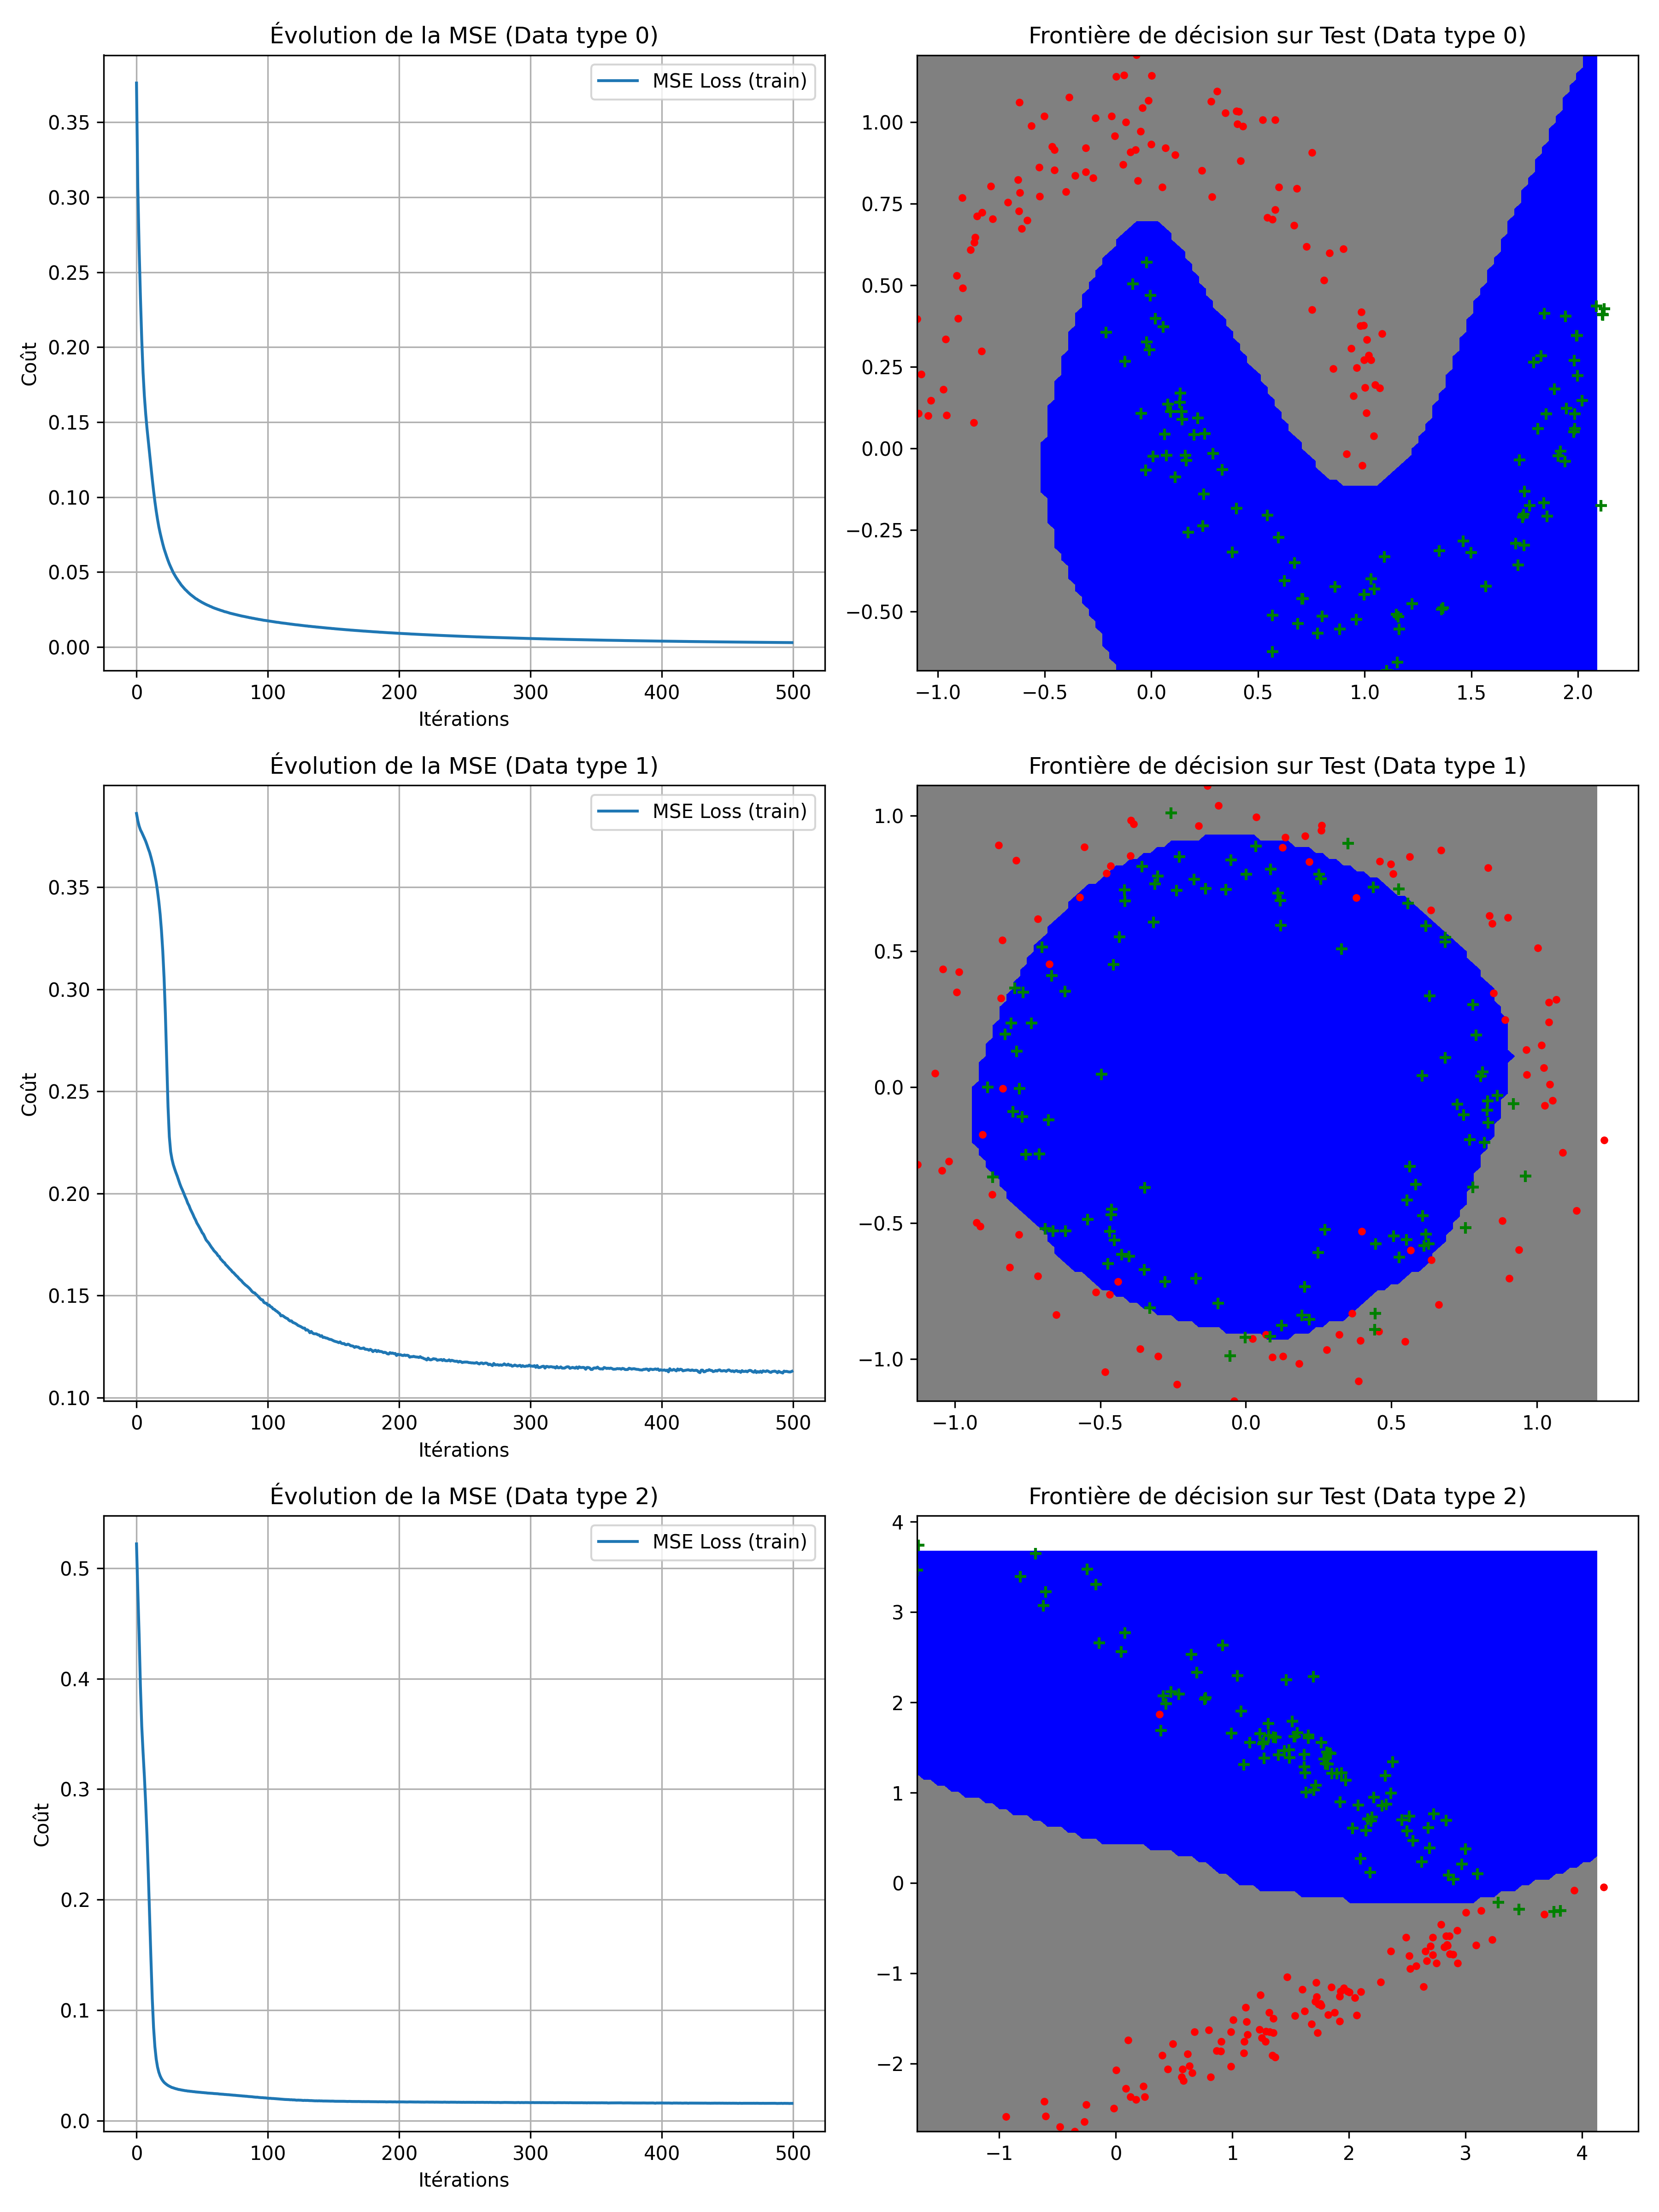
\includegraphics[width=0.8\linewidth]{Images/optim2.png}
    \caption{Loss et frontières avec optimisation (secondes données)}
	\label{fig:optim2}
\end{figure}

On remarque ainsi que nos notre loss atteint une valeur plus basse, améliorant légèrement les résultats grâce à l'utilisation de l'optimiseur.

\section{Mon quatrième est multi-classe}
On commence donc par implémenter notre module \textbf{SoftMax}, qui hérite donc de la classe module. On retranscrit ainsi la formule de la fonction softmax, en python, dans la méthode \textbf{forward}. De plus, afin de pouvoir gérer le multi-classe, on ajoute la perte cross-entropique, définie comme un maximum de vraisemblance. On prend ainsi soin d'éviter les valeurs nulles, afin de ne pas avoir de problème avec notre logarithme.
On expérimente ainsi sur de nouvelles données, celles des chiffres manuscrits, \textbf{USPS}. Les données sont déjà séparées en train et en test, il nous suffit donc d'entraîner notre modèle. Notre réseau de neurones est donc constitué de deux couches cachées, auxquelles on fini par appliquer un softmax. On utilise également la classe CrossEntropyLoss que nous venons de créer. Les résultats sont visibles dans la figure \ref{fig:multi1}.

\begin{figure}[H]
    \centering
    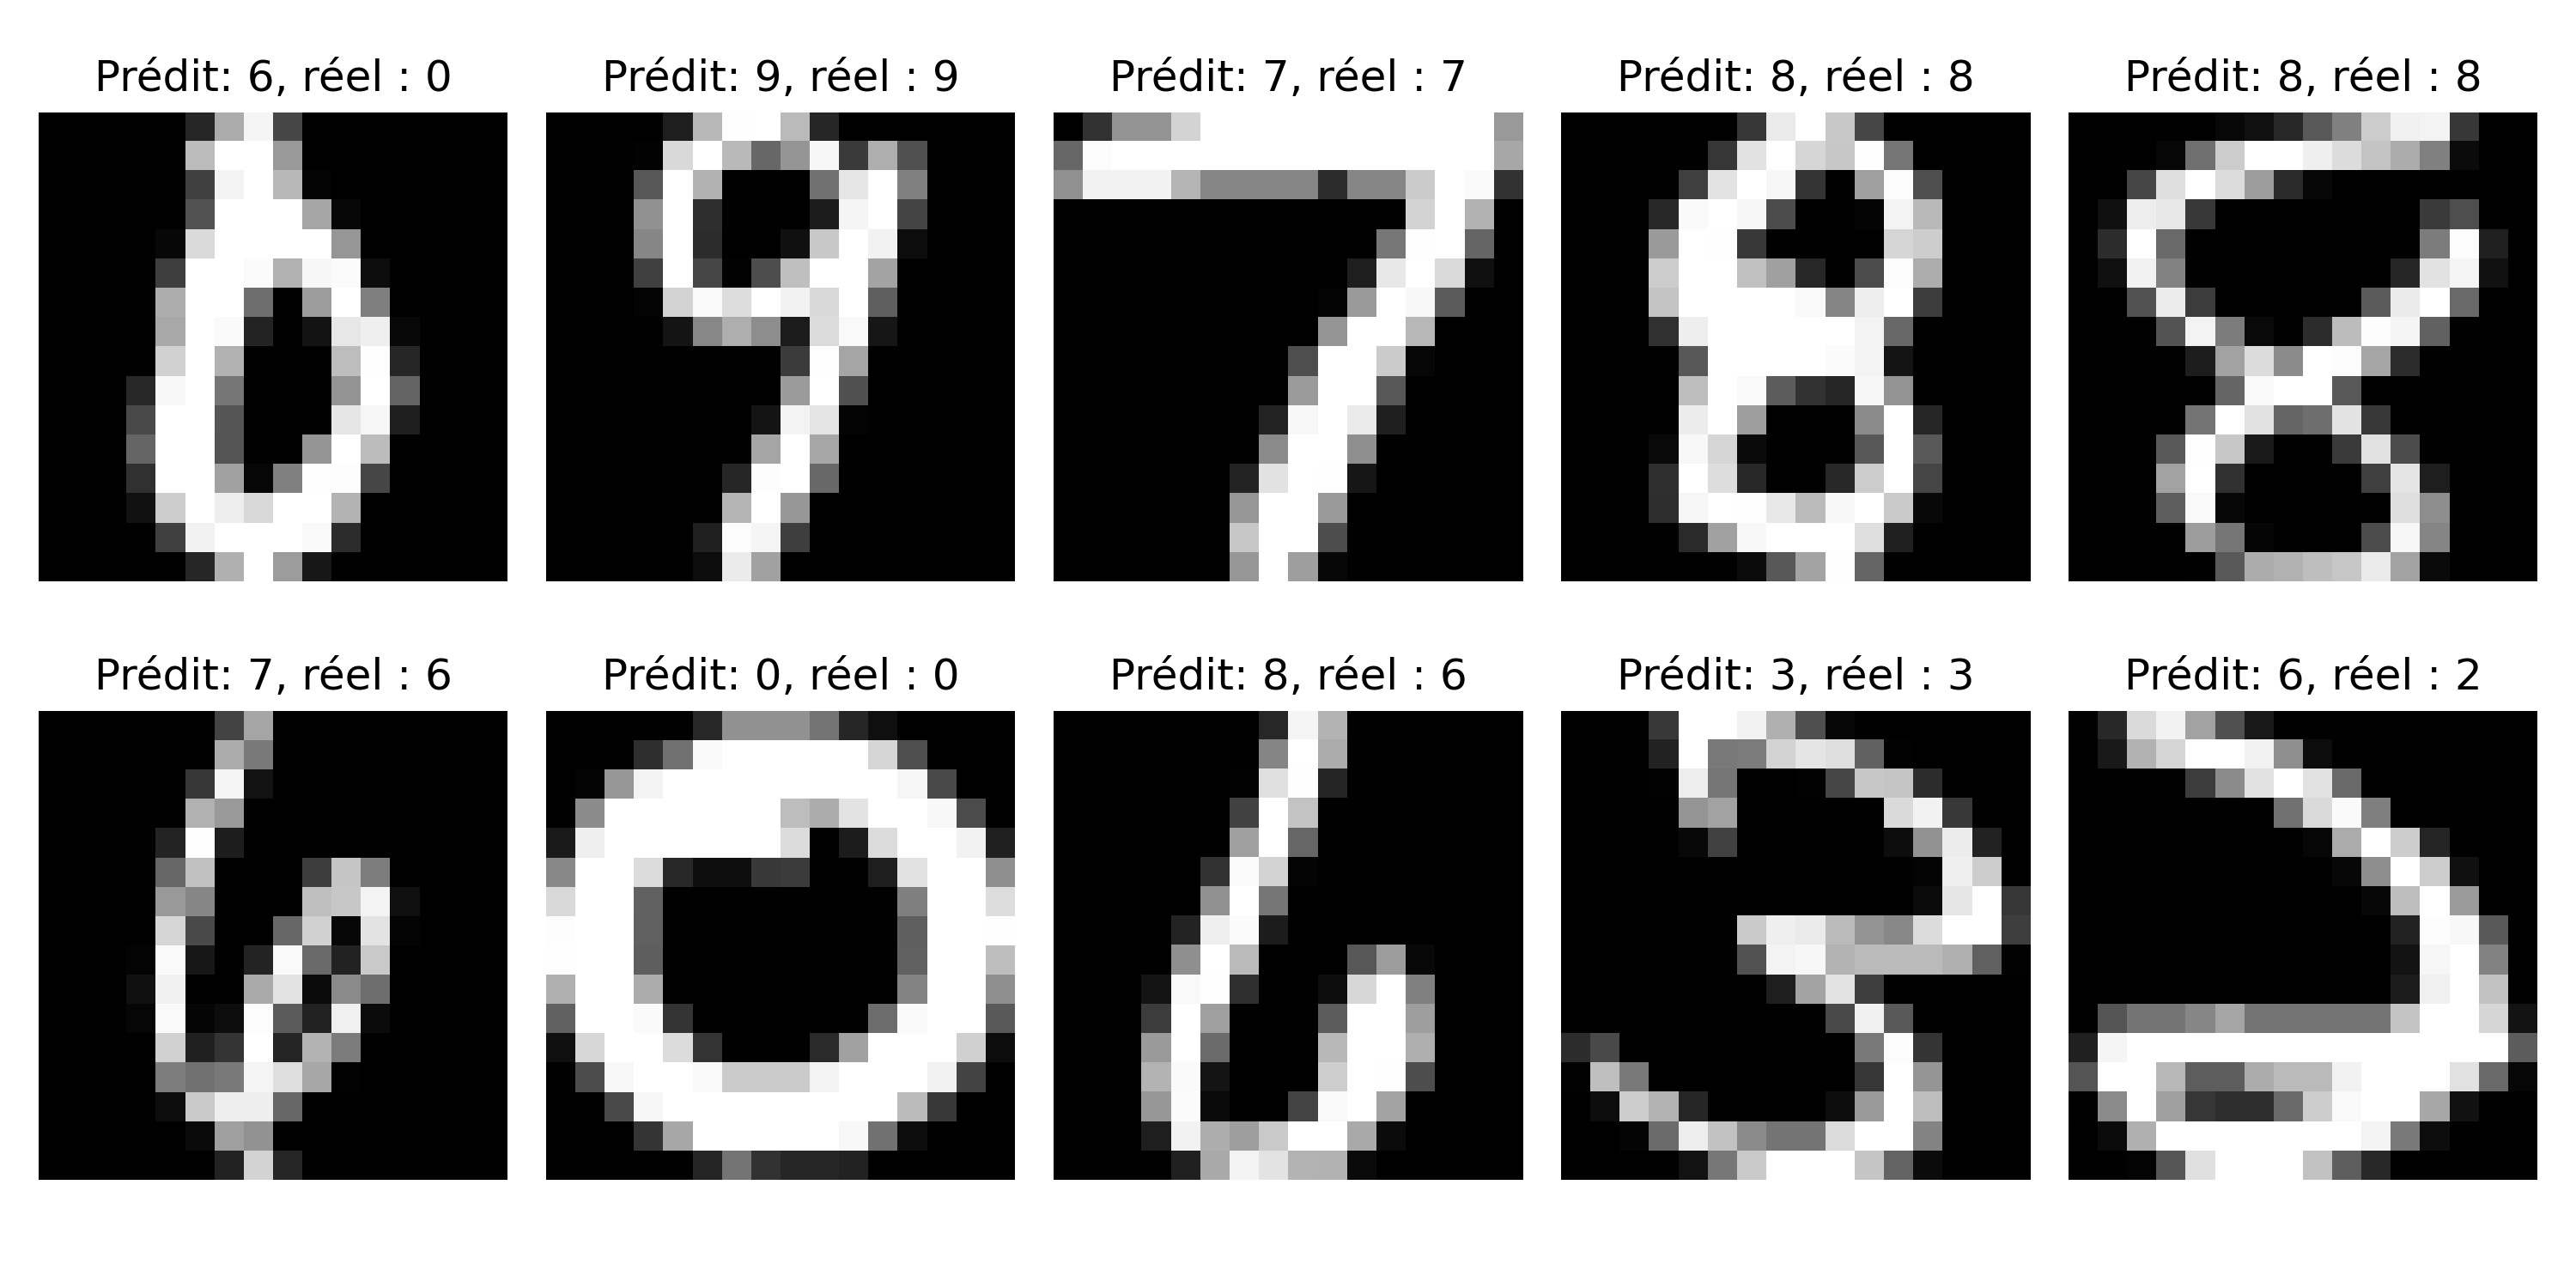
\includegraphics[width=0.8\linewidth]{Images/multi1.png}
    \caption{10 prédictions de la classification multi-classe (200 epochs)}
	\label{fig:multi1}
\end{figure}
En testant ainsi pour 200 epochs, on obtient une accuracy d'environ 78 \%, ce qui est un résultat plutôt encourageant. Les chiffres sont donc assez bien prédits, mais il reste encore environ 2 chiffres sur 10 qui sont mal classés. On peut améliorer ce résultat en utilisant la LogSoftMax et la LogCrossEntropy. Pour implémenter ces deux fonctions, on implémente simplement la Cross Entropy en intégrant le logsoftmax dans ces fonctions \textbf{forward} et \textbf{backward}. Lorsque l'on construit notre réseau, on ne met donc pas de fonction d'activation à la fin, celle-ci s'appliquant désormais directement lors du calcule de notre loss.
Les résultats exprérimentaux sont visibles dans la figure \ref{fig:multi2}.
\begin{figure}[H]
    \centering
    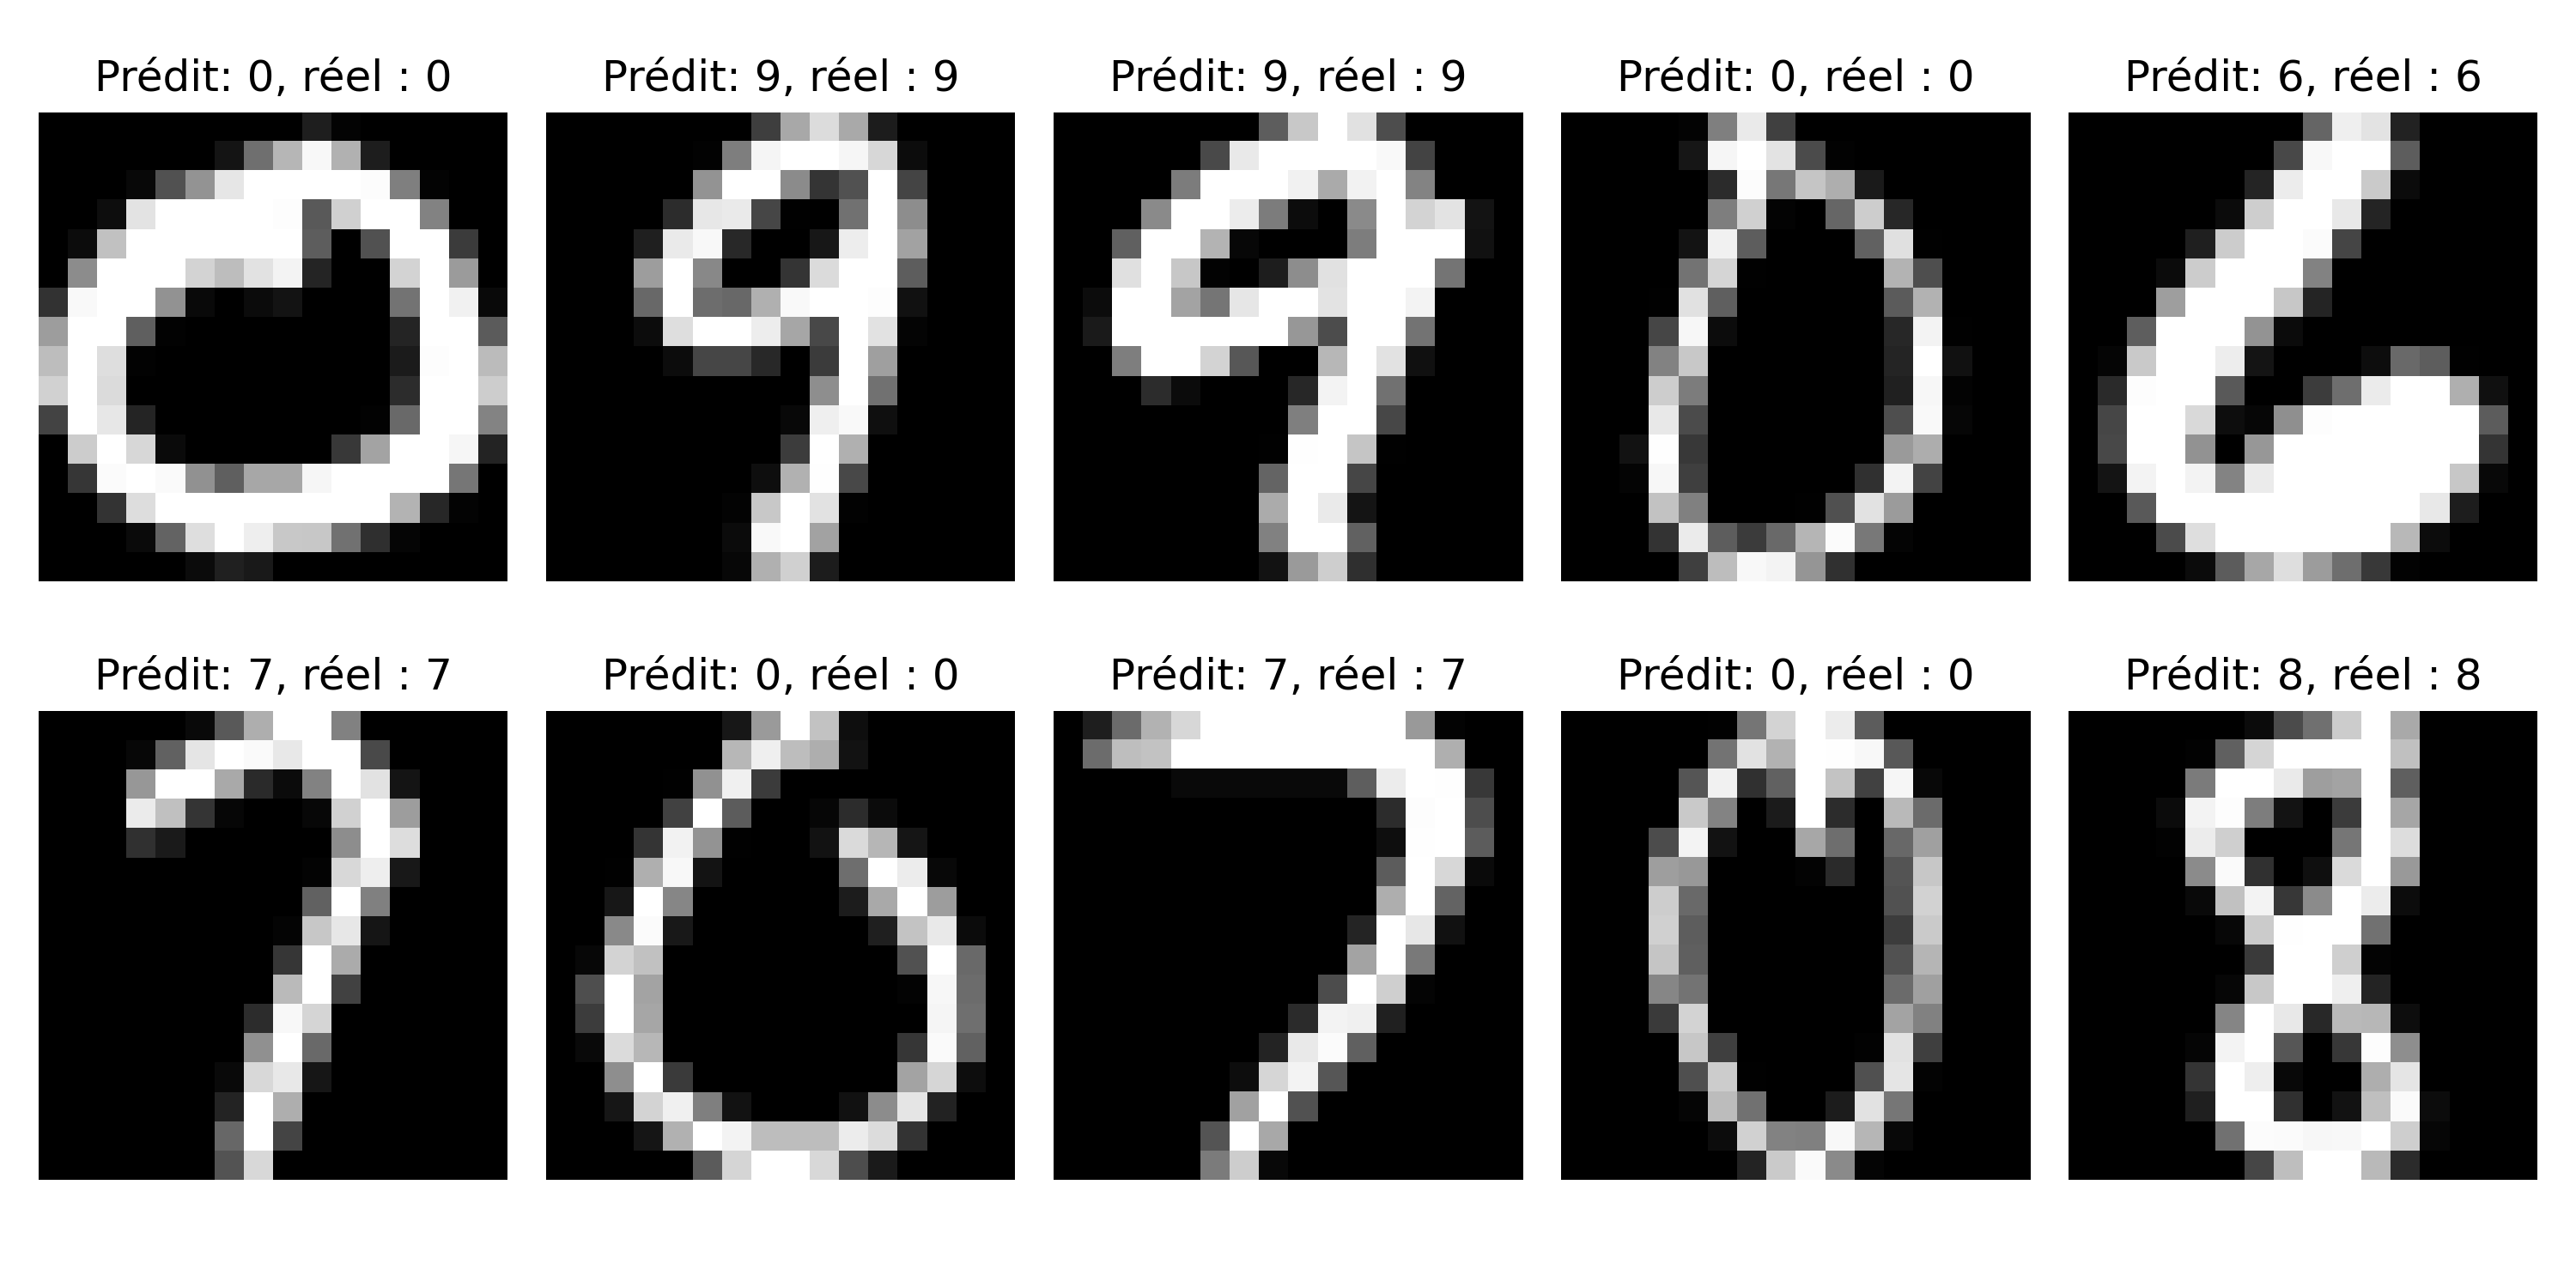
\includegraphics[width=0.8\linewidth]{Images/multi2.png}
    \caption{10 prédictions de la classification multi-classe (200 epochs)}
    \label{fig:multi2}
\end{figure}
Nous avons cette fois-ci une accuracy de 92 \%, ce qui montre l'efficacité de la LogCrossEntropy. Les chiffres sont ainsi en grande partie bien prédits, nous sommes donc désormais capables de résoudre des problèmes de classification multi-classe.


\section{Mon cinquième se compresse (et s'expérimente beaucoup)}
\subsection{Encodeur d'image de chiffre}
Nous allons donc mettre en place notre auto-encodeur. Pour cela, on modifie légèrement notre classe \textbf{Sequentiel}, afin de pouvoir construire un objet de cette classe à partir de deux autres objets de celle-ci.
Ceci va nous permettre de créer un réseau de type encodeur, puis un autre de type décodeur. Il suffit alors de construire l'objet \textbf{Sequentiel} en mettant les deux éléments dans une liste.
Notre réseau est alors construit de la manière suivante : 2 couches par partie de l'encodeur, la sortie de la première et l'entrée de la seconde étant en dimension 10, une pour chaque chiffre.

On crée ensuite notre \textbf{BCELoss}, en appliquant simplement la formule de celle-ci. Cela nous permettra d'obtenir de meilleures performances qu'avec la MSE.
On entraîne ensuite notre autoencodeur sur les données \textbf{USPS}, en utilisant la fonction d'optimisation SGD.
Les résultats sont visibles dans la figure \ref{fig:autoecodeur}.
\begin{figure}[H]
    \centering
    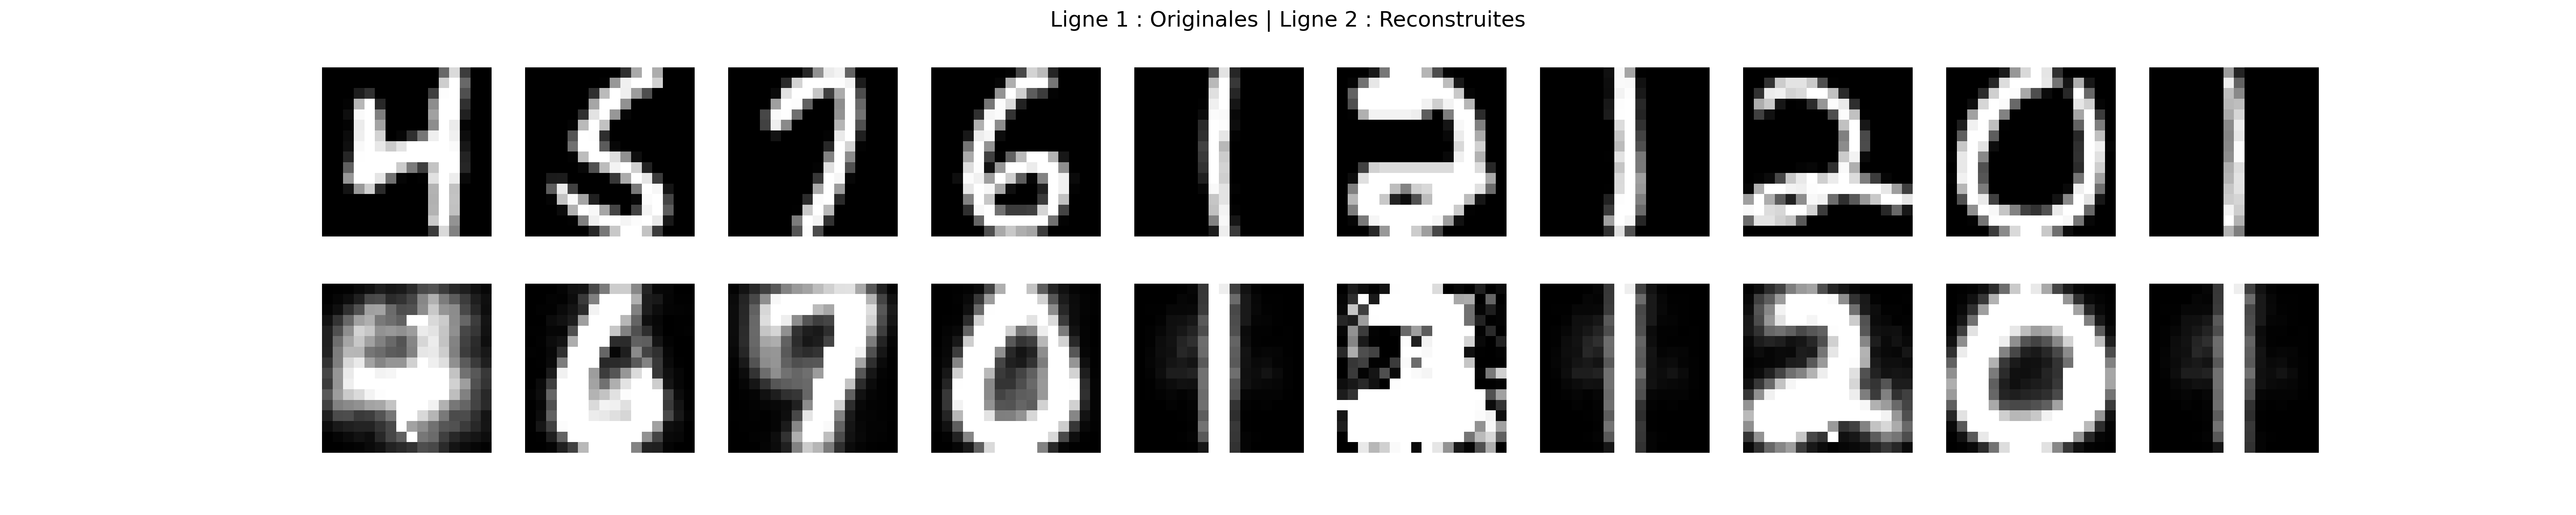
\includegraphics[width=1\linewidth]{Images/autoecodeur.png}
    \caption{10 prédictions de l'autoencodeur (1000 epochs)}
    \label{fig:autoecodeur}
\end{figure}
Parmi les 10 chiffres tirés au hasard, on remarque que certains sont très bien recréés, tandis que d'autres, comme le 5 et le 6, sont confondus avec d'autres chiffres.  Pour vérifier ce phénomène, on applique donc l'algorithme \textbf{TSNE}. Le résultat est visible dans la figure \ref{fig:tsne}.
\begin{figure}[H]
    \centering
    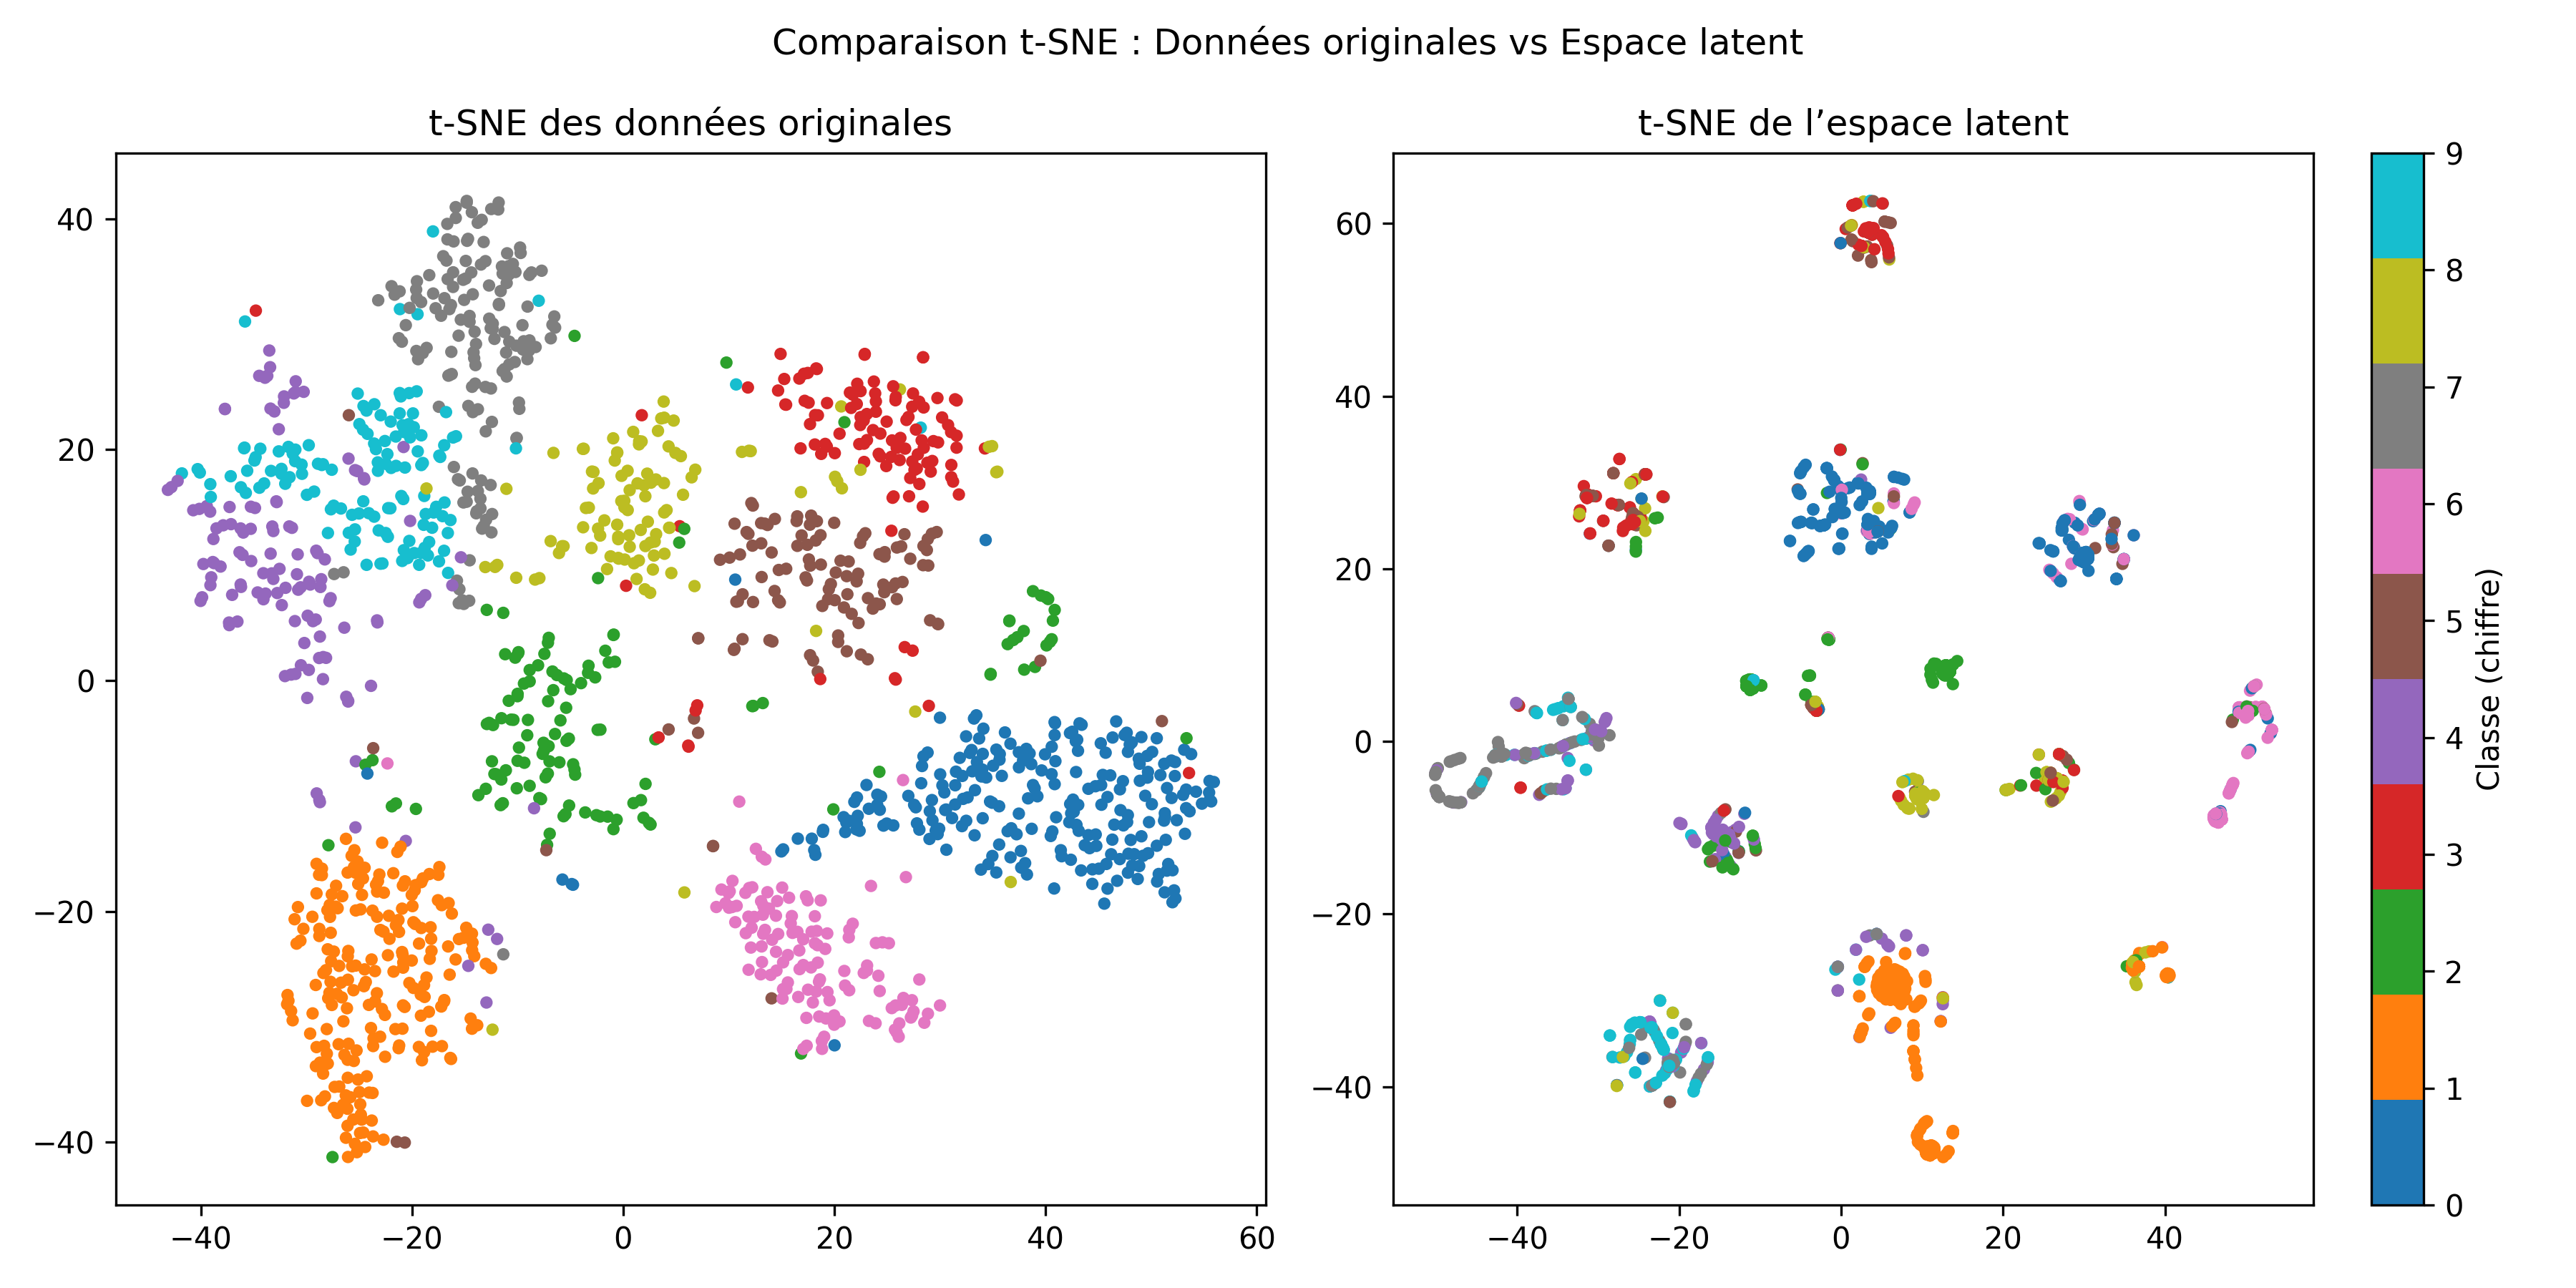
\includegraphics[width=0.8\linewidth]{Images/t-sne.png}
    \caption{Résultat de l'algorithme TSNE}
    \label{fig:tsne}
\end{figure}
On ajoute à cela un test avec les k-means, afin d'évaluer le clustering de nos chiffres manuscrits. Une représentation t-sne est visible dans le figure \ref{fig:k-means}. On peut voir que les clusters sont bien séparés, mais que certains de dissipent dans d'autres clusters, empêchant une reconstruction parfaite.
\begin{figure}[H]
    \centering
    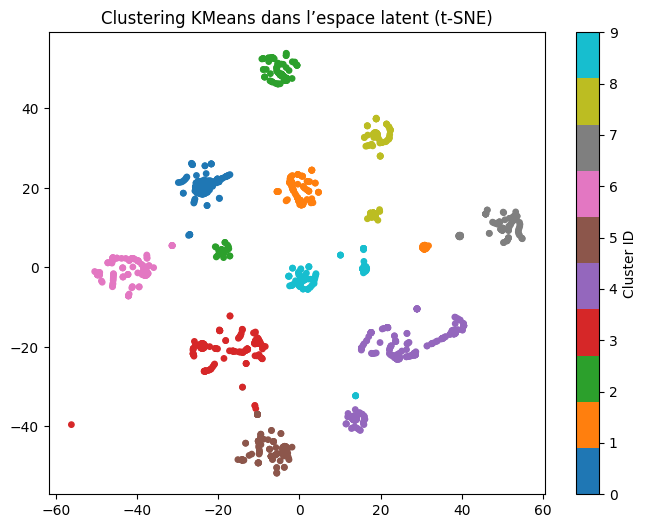
\includegraphics[width=0.8\linewidth]{Images/k-means.png}
    \caption{Résultat de l'algorithme K-means}
    \label{fig:k-means}
\end{figure}
En utilisant les métrique \textbf{Silhouette} et \textbf{ARI}, on a bien la confirmation de cette analyse : les clusters sont bien séparés mais ne sont pas alignés par rapport aux originaux.
On remarque ainsi que les clusters ne sont pas les mêmes, et que les chiffres dont les formes sont proches ont tendance à se mélanger dans l'espace latent, ce qui explique nos problèmes de reproduction totalement fidèle des chiffres.
Nous avons également mis en place une grid-search afin d'optimiser les valeurs des hyperparamètres pour le learning rate et la batch-size. Il s'est avéré que les meilleures valeurs étaient celles utilisées dans les expérimentations précédentes, du moins dans notre structure actuelle.

\subsection{Encodeur syntaxique de mot}

Nous avons choisi d’expérimenter l'architecture \textit{encodeur-décodeur} sur un problème linguistique, afin d’obtenir une représentation latente de mots français fondée uniquement sur leur forme orthographique. 
Notre hypothèse principale est la suivante : peut-on apprendre une représentation interne pertinente d’un mot à partir de sa seule structure (lettres et positions), sans recourir à une information sémantique ou contextuelle~?

3 Problématiques se sont posées :
\begin{itemize}
    \item Les vecteurs latents capturent-ils des propriétés linguistiques des mots, telles que le genre ou la fonction grammaticale~?
    \item Le décodeur est-il capable de reconstruire un mot correct à partir d’un mot bruité~?
    \item Peut-on utiliser cet espace latent comme prétraitement pour des tâches supervisées~?
\end{itemize}

\subsubsection{Donnée d'entraînement}

Nous avons utilisé le jeu de données Lexique3, qui regroupe environ 140,000 mots de la langue française accompagnés de leurs propriétés grammaticales. Ces informations sont particulièrement intéressantes pour évaluer la pertinence de l’espace latent appris par notre modèle.
\\ \\
Comme nous utilisons un réseau de type MLP, qui n’est pas conçu pour traiter des séquences de longueur variable, nous avons dû imposer certaines contraintes sur les données d’entraînement. En particulier, nous avons choisi de ne conserver que les mots de longueur fixe égale à cinq caractères, ce qui correspond approximativement à la longueur moyenne des mots les plus fréquemment utilisés en français.
\\ \\
Nous avons construit un alphabet composé de 39 caractères présents dans le corpus de mots. Chaque lettre est représentée par un vecteur one-hot, où chaque dimension correspond à un caractère de l’alphabet. À partir de cela, on peut représenter un mot comme une matrice composée de cinq vecteurs one-hot. Ce sont ces objets que notre modèle devra encoder et décoder.

\subsubsection{Protocole d'évaluation}

Afin d’évaluer la pertinence de la représentation latente apprise par notre autoencodeur, nous avons analysé plusieurs métriques et mené différentes expérimentations.
\\ \\
Nous nous sommes d’abord appuyés sur la valeur de la fonction de coût obtenue sur les données de test, en utilisant la \textit{Binary Cross Entropy}, définie précédemment, comme mesure de reconstruction.
\\ \\
Nous avons ensuite évalué la qualité de l’espace latent en l’utilisant comme entrée pour des classifieurs simples, en particulier des modèles de régression logistique. Ces classifieurs ont été entraînés sur différentes tâches de classification linguistique, telles que le genre grammatical ou le nombre (singulier/pluriel) des mots.
\\ \\
Pour mesurer l’apport de la représentation latente, nous avons comparé les performances des classifieurs lorsqu’ils sont entraînés à partir des représentations \textit{one-hot} versus celles issues de l’espace latent. Cette comparaison permet de déterminer si l’espace latent facilite ou non les tâches de classification, et donc s’il encode des propriétés linguistiques utiles.

\subsubsection{Expérimentation sans pré-traitement}

Nous avons commencé par définir un premier modèle d’autoencodeur appliqué à des mots de longueur fixe (5 lettres). La première observation notable fut la lenteur de l’apprentissage~: le modèle convergeait difficilement et présentait une forte tendance au sur-apprentissage. Le learning rate nécessaire est très élevé, cela s’explique sûrement par une mauvaise échelle initiale des poids, qui rend les gradients trop faibles pour produire des mises à jour significatives.
\\
Après avoir expérimenté différentes initialisations de poids, nous avons conclu que c’était la source du problème. L’utilisation de l’initialisation Xavier a permis une convergence bien plus rapide et de meilleures performances en test.
\\ \\
On utilise ici un réseau encoder \texttt{Linear(39*5, 50)} $\rightarrow$ \texttt{Linear(50, 10)} 
\\
et decoder : \texttt{Linear(10, 50)} $\rightarrow$ \texttt{Linear(50, 39*5)}

\begin{figure}[H]
    \centering
    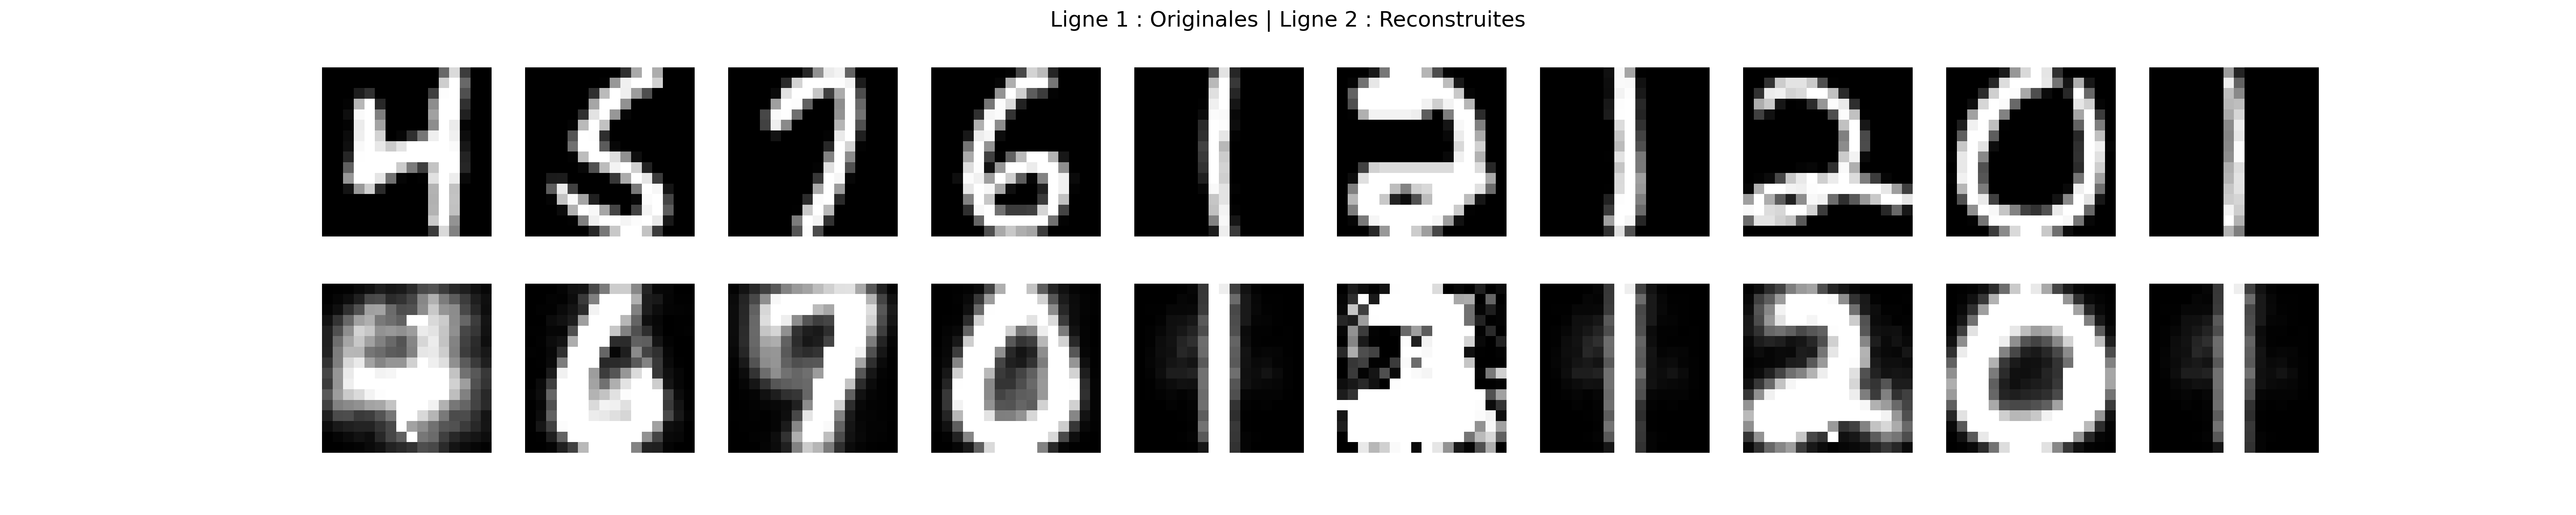
\includegraphics[width=0.7\textwidth]{Images/autoecodeur.png}
    \caption{Visualisation de l'architecture}
    \label{fig:mirror_example}
\end{figure}

\begin{figure}[H]
    \centering
    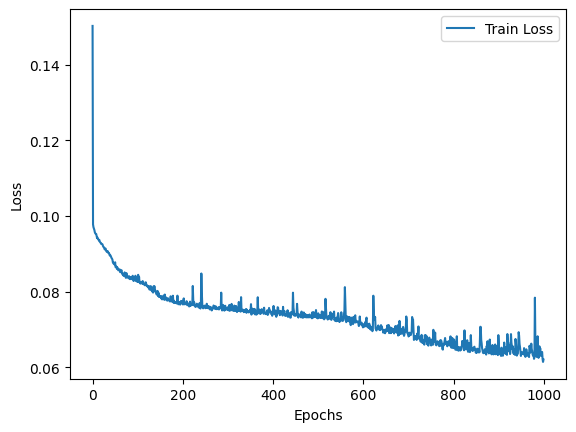
\includegraphics[width=0.6\linewidth]{Images/loss_no_init.png}
    \caption{Évolution de la loss pendant l’entraînement avec initialisation aléatoire standard}
    \label{fig:loss_no_init}
\end{figure}

\begin{figure}[H]
    \centering
    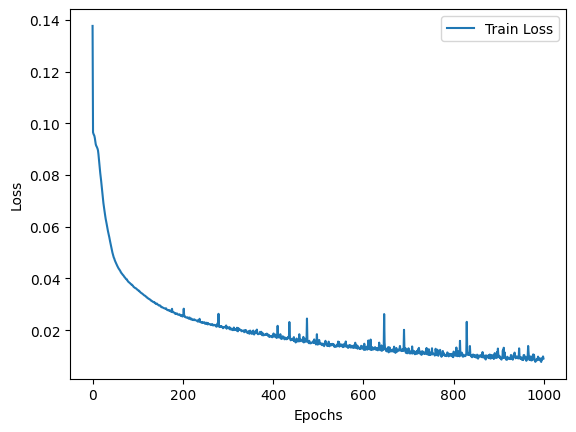
\includegraphics[width=0.6\linewidth]{Images/loss_xavier_init.png}
    \caption{Évolution de la loss pendant l’entraînement avec initialisation Xavier}
    \label{fig:loss_xavier_init}
\end{figure}

\begin{table}[H]
\centering
\begin{tabular}{lc}
\hline
\textbf{Modèle sur 1000 epoch} & \textbf{Loss en test} \\
\hline
Sans init (\texttt{np.random.randn}) & 0.0720 \\
Avec init Xavier & 0.0242 \\
\hline
\end{tabular}
\caption{Comparaison de la perte en test après 1000 époques selon l'initialisation des poids}
\end{table}

Malgré ces améliorations, le modèle reste très sensible au sur-apprentissage. Une réduction de la taille du réseau, en particulier de la dimension de l’espace latent, permet de limiter partiellement ce phénomène. Toutefois, l’équilibre entre sous-apprentissage et sur-apprentissage reste compliqué à atteindre.

\subsubsection{Ajout de bruit}

Afin de rendre le modèle plus robuste, nous avons introduit du bruit dans les données d’entraînement. Ce bruit est simulé par le remplacement aléatoire de certaines lettres d’un mot par d’autres lettres de l’alphabet choisies uniformément au hasard. Cette approche permet au modèle d’apprendre à reconstruire des mots partiellement corrompus, ce qui simule des erreurs telles que des fautes de frappe. De plus, cette technique agit comme une forme de régularisation, en réduisant le risque de surapprentissage sur les données d'entraînement. Pour introduire du bruit lors de l'entraînement, nous altérons, à chaque batch, une proportion globale des lettres définie par le paramètre \texttt{noise\_level}. Ainsi, certains mots peuvent ne subir aucune modification, tandis que d’autres peuvent être altérés à plusieurs reprises.


\begin{table}[H]
\centering
\begin{tabular}{lcccc}
\hline
\textbf{Train set} & \textbf{Loss train} & \textbf{Loss test (\texttt{noise\_level} = 0)} & \textbf{Loss test (0.1)} & \textbf{Loss test (0.2)} \\
\hline
Sans bruit & \textbf{0.0073} & 0.0242 & 0.0747 & 0.1061 \\
$\texttt{noise\_level} = 0.1$ & 0.0234 & \textbf{0.0131} & 0.0305 & 0.0451  \\
$\texttt{noise\_level} = 0.2$ & 0.0352 & 0.0148 & \textbf{0.0298} & \textbf{0.0411} \\
\hline
\end{tabular}
\caption{Comparaison de la perte en test et en train selon le niveau de bruit des données d'entraînement}
\end{table}

\begin{table}[H]
\centering
\begin{tabular}{lcc}
\hline
\textbf{Train set} & \textbf{PR Acc. train} & \textbf{PR Acc. test}  \\
\hline
Sans bruit & 54.06\% & 40.32\% \\
$\texttt{noise\_level} = 0.1$ & \textbf{90.4\%} & \textbf{72.83\%} \\
$\texttt{noise\_level} = 0.2$ & 87.69\% & 71.42\%  \\
\hline
\end{tabular}
\caption{Comparaison de la proportion de mot parfaitement reconstruit (PR) selon le set d'entraînement}
\end{table}

L’ajout de bruit permet au modèle de mieux généraliser, comme le montre les loss observées sur le train et test set. Sans bruit, les performances se dégradent sur les données de test, ce qui indique que le modèle a un peu overfitté.
\\ \\
Lorsqu’on introduit un peu bruit (\texttt{noise\_level}~$=0.1$), les performances de reconstruction s’améliorent nettement en test. Le modèle apprend à corriger des entrées bruitées, ce qui le pousse à produire des reconstructions plus stables et plus franches, même en présence de perturbations.
\\
On le voit aussi dans la proportion de mots parfaitement reconstruits. Le modèle sans bruit n’atteint que \textbf{54.06\,\%} de reconstruction exacte en entraînement, malgré une loss très basse. Nous avons émis l'hypothèse que la fonction de coût (Binary Cross Entropy) récompense des sorties proches de la vérité, mais pas forcément parfaitement binaires. En conséquence, le modèle sans bruit produit des sorties floues, qui minimisent bien la loss mais échouent plus souvent après seuillage à reconstruire le mot exact. Le bruit pousse le modèle à renvoyer des one-hot beaucoup plus tranché augmentant grandement la qualité de la reconstruction.
\\ \\
Enfin, assez logiquement le modèle entraîné sur des données plus bruitées (\texttt{noise\_level}~$=0.2$) arrive mieux à reconstruire en test sur des données bruitées.



\subsubsection{Masquage}

Toujours dans l’objectif d’améliorer la robustesse du modèle, nous avons également introduit un mécanisme de masquage. Celui-ci consiste à remplacer certaines lettres par un symbole spécial indiquant qu’une information est absente, dans notre cas nous avons décidé de les représenter avec un vecteur de lettre one-hot nul. Le modèle est alors entraîné à inférer les lettres manquantes en s’appuyant uniquement sur le contexte fourni par les autres lettres du mot. Cette approche favorise l’apprentissage des régularités internes et de la structure des mots.
\\ \\
En ce qui concerne la prédiction de caractères manquants, nous avons adopté deux approches pour évaluer la qualité de la reconstruction. Dans un premier temps, nous avons simplement observé le mot reconstruit par le modèle. Toutefois, lorsqu’un caractère est masqué dans un mot, plusieurs complétions valides peuvent exister. Par exemple, le mot partiellement masqué \texttt{b\_lle} peut correspondre à plusieurs solutions correctes telles que \textit{bulle}, \textit{balle}, \textit{belle} ou encore \textit{bille}. Pour pallier cette ambiguïté, nous avons adopté une approche basée sur les représentations latentes. Pour un mot comportant un caractère masqué, nous avons comparé sa représentation à celles des mots du vocabulaire complet encodé. Les mots dont les embeddings sont les plus proches (selon la distance euclidienne) sont alors considérés comme les reconstructions les plus plausibles.

\begin{table}[H]
\centering
\begin{tabular}{c|cc}
\hline
& \textbf{Entraînement 1} & \textbf{Entraînement 2}\\
\hline
\textbf{Mot encodé} & \multicolumn{2}{c}{\textbf{Mot reconstruit}}  \\
\hline
b\_lle & balle & bulle \\
b\_ule & boule & boule \\
\_\_\_\_\_ & barit & honie \\
\_\_r\_\_ & marie & héroe \\
\_\_q\_\_ & naque & hoque \\
q\_\_\_\_ & quici & quebe \\
\hline
\end{tabular}
\caption{Exemples de mots masqués reconstruit}
\end{table}

\begin{table}[H]
\centering
\begin{tabular}{l|cccc}
\hline
 & \multicolumn{2}{c}{\textbf{Entraînement 1}} & \multicolumn{2}{c}{\textbf{Entraînement 2}}\\
\hline
\textbf{Input} & \textbf{b\_lle} & \textbf{q\_\_\_\_} & \textbf{b\_lle} & \textbf{q\_\_\_\_}  \\
\hline
$1^{er}$ & balle & quant & balle & suffi \\
$2^{eme}$ & belle & quand & bulle & quand \\
$3^{eme}$ & bille & quête & bille & miaou \\
$4^{eme}$ & aille & queue & batte & quant \\
$5^{eme}$ & laque & ouate & balto & bémol \\
\hline
\end{tabular}
\caption{Classement des mots encodés du vocabulaire les plus proches (Distance euclidienne)}
\end{table}

On remarque que le modèle parvient à apprendre une structure assez convaincante. Par exemple, lorsqu’on lui masque toutes les lettres d’un mot, il est capable de générer des mots n’existant certes pas dans la langue française, mais néanmoins plausibles. On observe notamment un bon agencement des voyelles et des consonnes, ainsi que la présence de formes régulières en français, comme un t muet en fin de mot dans "barit" ou un ie final dans "honie". On constate le même phénomène avec le q qui est toujours suivi d'un u.
\\ \\
Pour le processus de plus proche voisin dans l'espace latent, le modèle parvient en général à obtenir des résultats pertinent. Néanmoins il reste des résultats peu cohérent, avec des mots proches dans l'espace latent assez loin de la structure du mot d'entrée.
\\ \\
Enfin ces expérimentations montrent la sensibilité du modèle à l'aléatoire de l'entraînement. En comparant les résultats de deux modèles identiques entraînés sur le même jeu de donnée on arrive à des résultat assez différent. Cela est probablement dû à l'entraînement par batch aléatoire et surtout par l'ajout de masque aléatoire dans l'entraînement.

\begin{table}[H]
\centering
\begin{tabular}{lcc}
\hline
\textbf{Train set} & \textbf{PR Acc. train} & \textbf{PR Acc. test}  \\
\hline
$\texttt{noise\_level} = 0.1$ & \textbf{90.4\%} & \textbf{72.83\%} \\
$\texttt{mask\_level} = 0.1$& 83.19\% & 61.33\%  \\
$\texttt{mask\_level} = 0.2$& 83.15\% & 68.16\%  \\
\hline
\end{tabular}
\caption{Comparaison de la proportion de mot parfaitement reconstruit (PR) selon le set d'entraînement}
\end{table}

L'ajout de bruit reste le processus qui aide le mieux le modèle à généraliser une bonne reconstruction.


\subsubsection{Padding}

Grâce au processus de masquage, nous avons pu expérimenter l’encodage de mots de longueur variable. Nous fixons une longueur maximale (choisie ici comme 10), et lorsqu’un mot est plus court, nous ajoutons autant de caractères de masquage que nécessaire pour atteindre cette longueur. Cela permet de conserver une représentation de taille fixe, tout en traitant des mots de tailles différentes. L’objectif de cette expérience est de déterminer si le modèle est capable de généraliser à des mots de longueur variable, et plus précisément, s’il parvient à apprendre à masquer lui-même la fin du mot lorsque celle-ci ne contient plus d’information pertinente. On utilise encore le processus de bruitage des données, cette fois seulement sur les lettres pas masquées.


\begin{table}[H]
\centering
\begin{tabular}{cc}
\hline
\textbf{Mot encodé} & \textbf{Mot reconstruit}\\
\hline
pilule & pilulerxàc \\
marque & marquertat \\
apprendre & apprentrez \\
ordinateur & artinatern \\
chat & chatreszzi \\
\hline
\end{tabular}
\caption{Exemples de mots paddé reconstruit}
\end{table}

Le modèle n'arrive pas à masquer la fin du mot, il génère systématiquement une suite de lettre de taille 10. Les mots courts, de taille inférieur à 6 sont plutôt bien reconstruit, outre les lettres qui dépasse. Cependant les mots plus longs ont plus de difficulté à être reconstruit complètement. En conclusion ce modèle est inutilisable pour cette tâche. 
\\ \\
Étant donné que le modèle ne semble pas capable de masquer correctement la fin d’un mot, nous avons envisagé plusieurs pistes pour contourner ce problème. L’une des solutions consiste à faire prédire par le modèle, en plus de la reconstruction du mot, sa longueur sous forme d’un vecteur one-hot de taille 10. En plus de cela pour le rendre plus robuste, on propagerait la loss uniquement sur les sorties correspondant aux positions effectivement présentes dans le mot, en ignorant les caractères de remplissage.  
Par manque de temps, nous n’avons pas pu expérimenter ces alternatives.

\subsubsection{Résultats}

À l’image des visualisations classiques sur des images de chiffres, nous avons projeté les représentations latentes des mots dans un espace 2D à via la méthode t-SNE. L’objectif était d’observer si des clusters distincts se formaient en fonction de certaines propriétés linguistiques, notamment le genre grammatical et le nombre.

\begin{figure}[H]
    \centering
    \begin{minipage}[b]{0.32\textwidth}
        \centering
        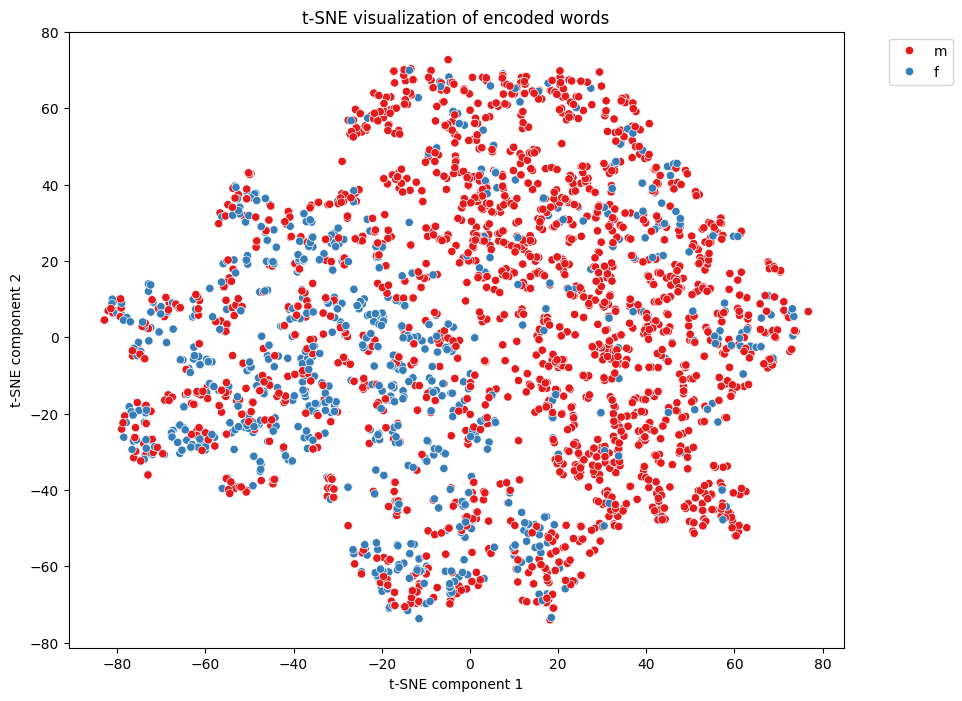
\includegraphics[width=\textwidth]{Images/tsne_mf.png}
        \caption*{(a) Masculin / Féminin}
        \label{fig:mf}
    \end{minipage}
    \hfill
    \begin{minipage}[b]{0.32\textwidth}
        \centering
        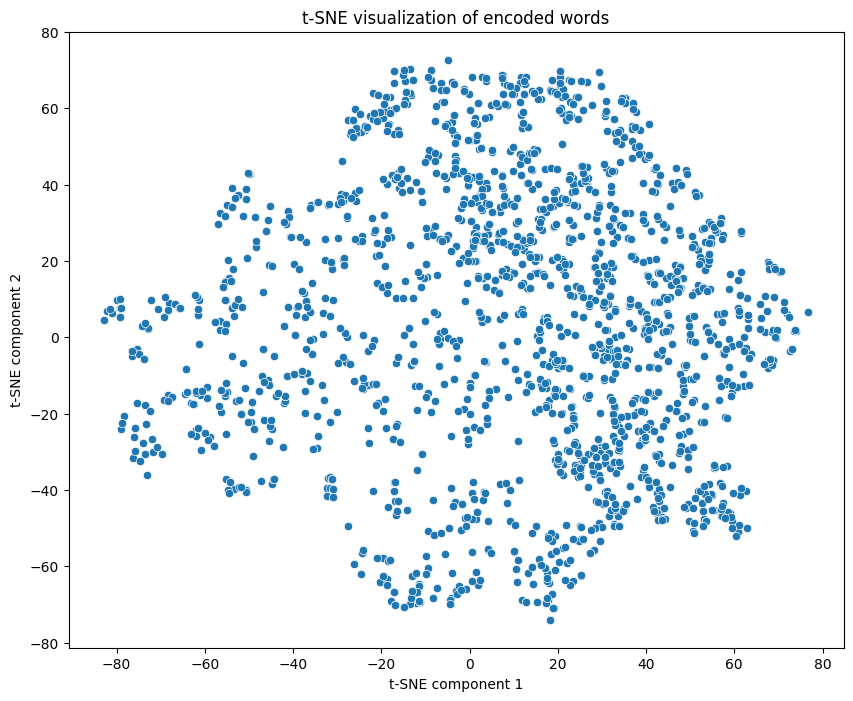
\includegraphics[width=\textwidth]{Images/tsne_m.png}
        \caption*{(b) Masculin}
        \label{fig:m}
    \end{minipage}
    \hfill
    \begin{minipage}[b]{0.32\textwidth}
        \centering
        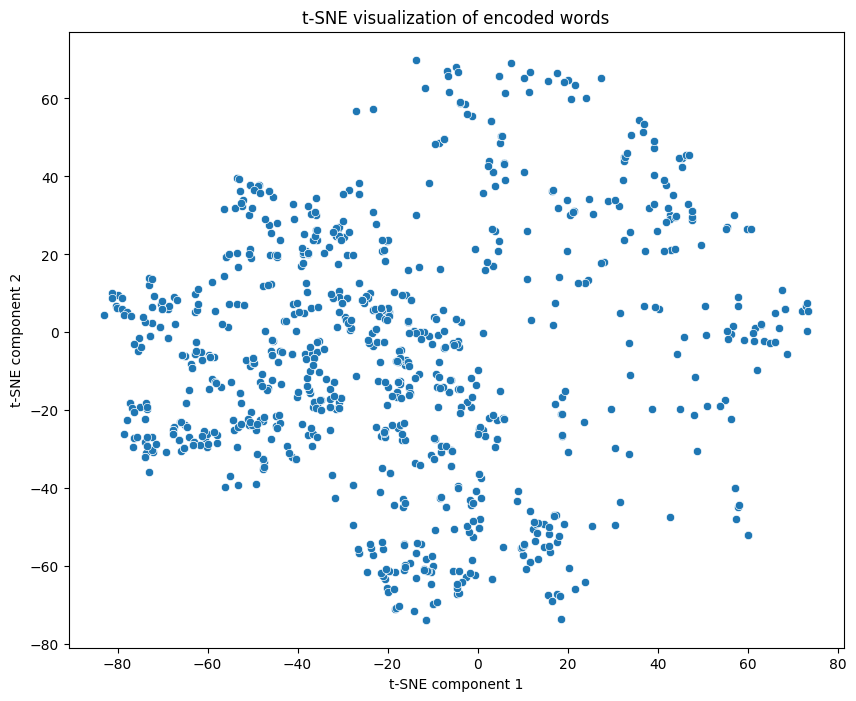
\includegraphics[width=\textwidth]{Images/tsne_f.png}
        \caption*{(c) Féminin}
        \label{fig:f}
    \end{minipage}
    \caption{Visualisation t-SNE des représentations latentes selon le genre grammatical.}
    \label{fig:tsne_genre}
\end{figure}

On peut observer pour le genre qu'à défaut d'avoir des clusters bien distinct, on a tout de même une séparation sur la distribution des points selon leur genre. Avec ce run, les points masculins sont plus dense sur la composante 1 positif, pour les féminins ils sont plus répandus sur la composante 1 dans les négatifs. Cela supposerais qu'il y aurait donc bien une séparation entre féminin et masculin à partir de la structure des mots. Il est possible que cela représente sûrement les cas très disciminant (-e présent à la fin des mots féminins...).

\begin{table}[H]
\centering
\begin{tabular}{lcc}
\hline
 & \textbf{Acc. Test Genre} & \textbf{Acc. Test Nombre} \\
\hline
One-hot & 88.64\% & 100\% \\
Sans bruit & 76.77\% & 96.64\% \\
$\texttt{noise\_level} = 0.1$ & 81.21\% & 98.6\% \\
\hline
\end{tabular}
\caption{Comparaison des performances en test de régressions logistique selon le format des données}
\end{table}

La représentation one-hot permet d’obtenir de meilleurs résultats que l’espace latent pour les tâches de classification. Cela peut s’expliquer par le fait que l’autoencodeur tend à produire des représentations plus compactes mais aussi plus floues. Pour des tâches relativement simples comme la prédiction du genre ou du nombre d’un mot, la précision brute de la représentation one-hot reste plus efficace.
\\ \\
Nos expérimentations ont montré qu’une perte de reconstruction faible n’impliquait pas nécessairement de meilleures performances en classification. Par ailleurs, de nombreux mots peuvent être considérés comme triviaux pour la prédiction du genre grammatical (par exemple, un mot masculin ne se terminant pas par un -e, ou un mot féminin se terminant par un -e). Sur les cas non-triviaux (par exemple: guide), tous les modèles obtiennent de moins bons résultats. Toutefois, certains entraînements d’autoencodeurs ont parfois réussi à surpasser la représentation one-hot, montrant que l’espace latent reste capable de capturer des propriété pertinentes selon les conditions d’apprentissage.
\\ \\
En conclusion, l’autoencodeur appliqué à des mots sur la base de leur structure syntaxique s’est révélé capable de produire une représentation latente partiellement pertinente. Les différentes expériences menées, notamment le masquage de caractères, ont permis de mettre en évidence sa capacité à mémoriser des formes syntaxiques régulières de la langue Française.
\\
Pour le débruitage l'architecture est assez performantes, elle peut être utilisé comme une solution légère pour débruiter un mot sans base de donnée. Cependant des algorithmes déterministes utilisant la base de données complète reste quand même plus performants.
\\ \\
L’approche par MLP a considérablement limité les performances de l’encodage, notamment en raison de son incapacité à exploiter la structure séquentielle des mots. En traitant chaque mot comme un simple vecteur plat, le modèle ne peut pas capturer efficacement les dépendances entre lettres ni la position relative des caractères. Une architecture récurrente ou à base d’attention, comme les RNN ou les Transformers, reste plus adaptée pour encoder des informations structurelles plus fines et améliorer la qualité des représentations latentes.
\\ \\

\subsubsection{Expérimentations supplémentaires}
On a implémenté deux modules supplémentaire qu'on a pas inclus dans ce rapport, on a malheureusement pas eu assez de temps pour obtenir des résultats concluants. Leur objectif commun était d'apprendre une représentation latente des lettres avant d'utiliser leur représentation dans un encodeur de mot. 
\\ \\
Le premier modèle encode chaque lettre à l’aide d’un encodeur distinct pour chaque position dans le mot, permettant ainsi d’apprendre une représentation contextuelle spécifique à chaque emplacement. Le second modèle, plus contraint, apprend un unique encodeur partagé pour toutes les lettres, quelle que soit leur position. On a obtenu des convergences vers des loss trop élevé les rendant peu utilisable. Il s'agit certainement d'un problème d'implémentation.


\end{document}
